\documentclass[a5paper,10pt,twoside,twocolumn]{memoir}
\usepackage[total={138mm,180mm}, papersize={148mm,210mm},left=5mm,top=10mm]{geometry}
\usepackage[czech]{babel}
\usepackage[utf8]{inputenc}
\usepackage{graphicx}

\title{Kytice}
\author{Karel Jaromír Erben}
\date{\today}

\begin{document}

\newgeometry{left=15mm,total={118mm,180mm}}

\maketitle
\thispagestyle{empty}
\newpage

\tableofcontents*
\thispagestyle{empty}

\setlength{\versewidth}{\textwidth}
\renewcommand{\PoemTitlefont}{\normalfont\sffamily\hspace{\vleftmargin}}
\pagestyle{plain}
\newpage
\PlainPoemTitle

\restoregeometry

~

\newpage

\newpage

\begin{figure*}[p]
\centering
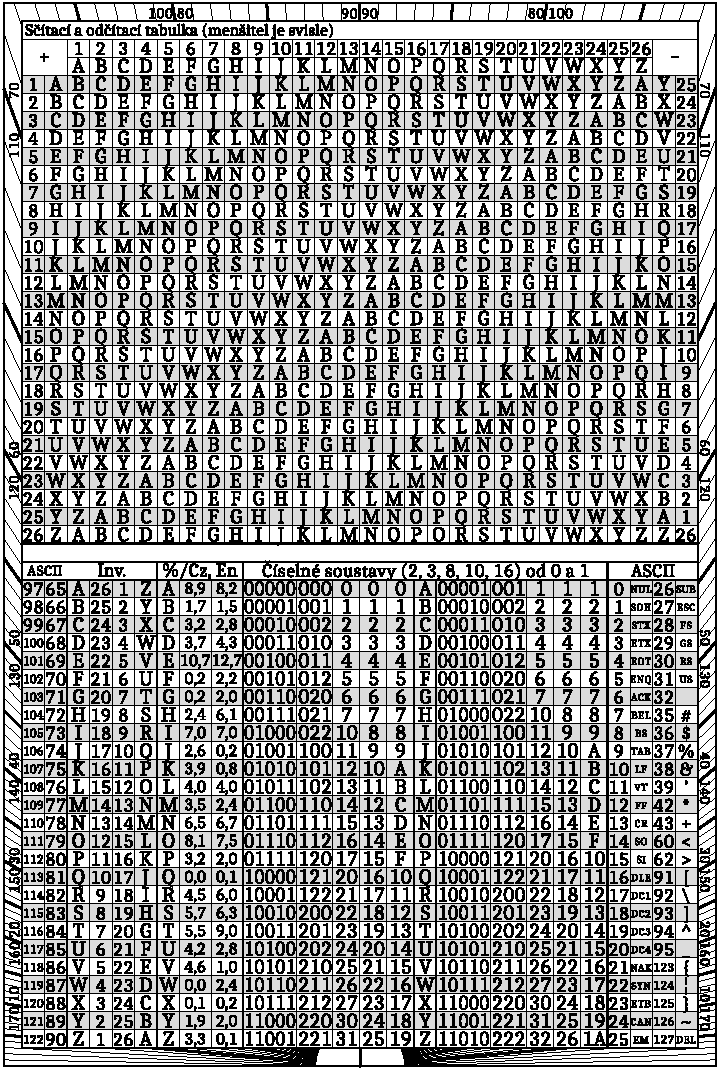
\includegraphics{pomucky/p1.pdf}
\end{figure*}

\begin{figure*}[p]
\centering
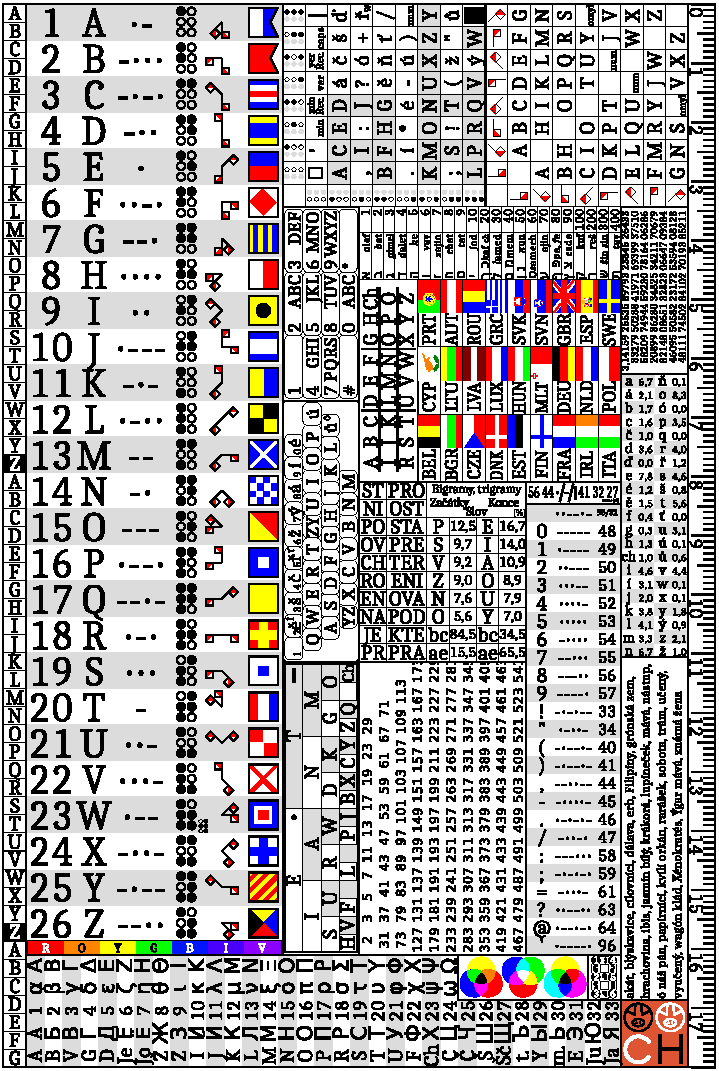
\includegraphics{pomucky/p2.pdf}
\end{figure*}



\PoemTitle{Kytice}
\begin{verse}
Zemřela matka a do hrobu dána, \\
siroty po ní zůstaly; \\
i přicházely každičkého rána \\
a matičku svou hledaly.
\end{verse}

\begin{verse}
I~zželelo se matce milých dítek; \\
duše její se vrátila \\
a vtělila se v~drobnolistí kvítek, \\
jím mohylu svou pokryla.
\end{verse}

\begin{verse}
Poznaly dítky matičku po dechu, \\
poznaly ji a plesaly; \\
a prostý kvítek, v~něm majíc útěchu, \\
mateřídouškou nazvaly. --
\end{verse}

\begin{verse}
Mateřídouško vlasti naší milé, \\
vy prosté naše pověsti, \\
natrhal jsem tě na dávné mohyle -- \\
komu mám tebe přinésti?
\end{verse}

\begin{verse}
Ve skrovnou já tě kytici zavážu, \\
ozdobně stužkou ovinu; \\
do šírých zemí cestu ti ukážu, \\
kde příbuznou máš rodinu.
\end{verse}

\begin{verse}
Snad se najde dcera mateřina, \\
jí mile dech tvůj zavoní; \\
snad že i najdeš některého syna, \\
jenž k~tobě srdce nakloní!
\end{verse}
\PoemTitle{Poklad}

\begin{verse}
I~\end{verse}

\begin{verse}
Na pahorku mezi buky \\
kostelíček s~věží nízkou; \\
z~věže pak slyšeti zvuky \\
hájem a sousední vískou. \\
Není zvuk to zvonka jemný, \\
tratící se v~blízké stráně: \\
dřevatě to rachot temný, \\
zvoucí lid do chrámu Páně. \\
A~tu z~vísky k~boží slávě \\
vzhůru běží zástup hojný: \\
veský lid to bohabojný, \\
a dnes Velký pátek právě. \\
V~chrámě truchlo: holé stěny; \\
oltář černá rouška kryje, \\
na roušce kříž upevněný; \\
v~kůru zpívají pašije. \\
A~hle, co se bělá v~lese, \\
v~černém lese za potokem
\end{verse}

\begin{verse}
Nějaká to veská žena, \\
ana v~náručí cos nese. \\
I~jde rychlým žena krokem, \\
svátečně jsouc oblečena, \\
tam tou strání za potokem -- \\
pacholátko malé nese.
\end{verse}

\begin{verse}
Běží žena, dolů běží, \\
pospíchá do chrámu Páně: \\
tu nablízku lesní stráně \\
kostel na pahorku leží. \\
A~v~úvale ku potoku \\
náhle ubystřuje kroků; \\
neb jak větřík volně věje, \\
z~kostela slyšeti pění: \\
v~kůru tam se právě pěje \\
Krista Pána umučení. \\
Běží, běží podle skály: \\
„Co to? Mám-li věřit oku? \\
Což mě moje smysly šálí?“ \\
Stane, ohlíží se kolem -- \\
rychle kroky zpět obrací, \\
stane zase, zas se vrací -- \\
„Tam ten les, a zde ty klesty, \\
tamto vede cesta polem -- \\
vždyť jsem nezbloudila z~cesty! \\
Bože, co se se mnou děje! \\
Což zde nejsem u~kamena? \\
Jaká se tu stala změna!“ \\
Zase stojí, zase spěje, \\
celá jsouci udivena, \\
oči rukou si protírá, \\
o~krok blíže se ubírá: \\
„Bože, jaká to tu změna!"
\end{verse}

\begin{verse}
Tu, kde z~divokého klestu, \\
od kostela tři sta kroků, \\
veliký čněl kámen v~cestu, \\
co se nyní jeví oku? \\
Jeví se tu ženě, jeví \\
vchodem vršek otevřený -- \\
vysvětliti sobě neví -- \\
kámen v~cestu postavený, \\
postavena celá skála \\
jak by od věků zde stála. \\
Jeví se tu, jeví ženě \\
chodba pod zemí, co síně \\
vyklenutá ve křemeně; \\
a tam, klenba kde se tratí, \\
ve tmavém pahorku klíně, \\
jakýs plamen znamenati. \\
I~hoří to jasnoběle, \\
jako v~noci svit měsíčka; \\
i zaplává rudoskvěle, \\
jak by západ to sluníčka.
\end{verse}

\begin{verse}
I~vidouc to žena žasne \\
a ke vchodu až pokročí, \\
a zastíníc dlaní oči, \\
hledí v~ono místo jasné. \\
„Bože, jak se to tam svítí!“ \\
Oči rukou si protírá, \\
o~krok blíže se ubírá: \\
„Jak se to tam divně svítí! \\
Co to asi může býti?“ \\
Dále jíti však se bojí, \\
hledíc tam, a venku stojí. \\
A~co váhá a co stojí, \\
v~klenbu patříc neustále, \\
mizí bázeň za pohledem, \\
zvědavost ji pudí předem, \\
a žena se béře dále. \\
Krok za krokem -- a vždy dále \\
mocně ji to jíti pudí; \\
krok za krokem -- a ve skále \\
jen se spící ohlas budí. \\
A~čím dál přichází žena, \\
stále divná roste záře. \\
Již již končí se sklepení; \\
avšak žena omráčena \\
rukou zakrývá si tváře, \\
přímo patřit možné není. \\
Vidí, vidí -- co zde vidí, \\
kdy to viděl který z~lidí? \\
Tolik krásy, tolik blesku \\
mní uzříti jen v~nebesku!
\end{verse}

\begin{verse}
Dvéře tu jsou otevřeny \\
do nejskvělejšího sálu; \\
zlatem jen se svítí stěny, \\
strop rubíny vyložený, \\
pod ním sloupy ze křišťálu. \\
Z~obojí pak strany dveří \\
na podlaze mramorové -- \\
kdo neviděl, neuvěří -- \\
hoří, hoří dva ohňové; \\
dva ohňové tuto hoří, \\
nic jich blesku neumoří: \\
nade stříbrem po levici \\
lunou oheň vzhůru plane, \\
nade zlatem po pravici \\
sluncem pláti neustane. \\
Planou ohně, jizba plane, \\
obalena září jasnou; \\
a dokud tu poklad stane, \\
plamenové nevyhasnou, \\
nic jich blesku neumoří.
\end{verse}

\begin{verse}
Na prahu tu žena stojí, \\
celá stojí oslepena; \\
očí pozdvihnout se bojí, \\
nemůž zříti do plamena. \\
Na levici dítě nese, \\
pravou levé mne si oko; \\
a když trochu ohlídne se, \\
osmělí a vzpamatuje, \\
vzdychne sobě přehluboko \\
a tak v~duši své rokuje: \\
„Milý bože, co já zkusím \\
na tom světě nouze, hladu! \\
Bídně život chránit musím -- \\
a zde tolik těch pokladů! \\
Tolik stříbra, tolik zlata \\
v~podzemní tu leží skrejši! \\
Jenom hrstku z~té hromady -- \\
a já byla bych bohata, \\
a byla bych nejšťastnější, \\
já i moje dítě tady!"
\end{verse}

\begin{verse}
A~co myslí a co stojí, \\
ohroženější se stane; \\
svatým křížem se ozbrojí \\
a jde, kde to běle plane. \\
Jde a stříbra kousek zdvihne, \\
avšak zase tam položí; \\
zdvihne zas a je prohlíží, \\
jeho blesk a jeho tíži -- \\
a zdali je zas položí? \\
Ne, již v~klíně jí se mihne. \\
A~zdařením tím smělejší: \\
„Jistě toto prst je boží, \\
poklad ukázal mi v~skrejši, \\
chce, bych byla oblažena: \\
i zhřešiti bych musela, \\
bych jím pohrdnouti měla!"
\end{verse}

\begin{verse}
Takto k~sobě mluvíc žena, \\
chlapce na zem z~ruky složí, \\
klekne a klín rozestírá, \\
chutě z~hromady nabírá \\
a do klína stříbro skládá: \\
„Jistě toto prst je boží, \\
jenž nás obohatit žádá!“ \\
Béře, béře ze hromady -- \\
klín již plný, sotva vstává, \\
ještě v~šátek sobě dává, \\
tak ji mámí stříbra vnady! \\
A~když již chce odtud jíti: \\
ach, zde ještě pacholete! \\
Jak je ke vší tíži vzíti?
\end{verse}

\begin{verse}
Pacholátko již dvouleté; \\
vysypati zase štěstí \\
nezdá se jí dobré býti; \\
obého pak nemůž nésti.
\end{verse}

\begin{verse}
A~hle, stříbro matka nese! \\
Dítě se tu na ni třese: \\
„Mama!“ volá, „mama, mama!“ \\
chytajíc ji ručinkama. \\
„Mlč, synáčku, mlč, mlč, hochu, \\
počkej tuto jenom trochu, \\
hned tu bude zase mama!“
\end{verse}

\begin{verse}
A~již běží, síní běží, \\
již i síně za ní leží; \\
přes potok, po stráni k~lesu \\
spěchá žena ve svém plesu. \\
A~než malá ušla chvíle, \\
prázdná zpátky zas pospíchá; \\
a ve potu, sotva dýchá, \\
stane zase již u~cíle.
\end{verse}

\begin{verse}
A~jak vítr zlehka věje, \\
z~kostela slyšeti pění: \\
v~kůru tam se právě pěje \\
Krista Pána umučení.
\end{verse}

\begin{verse}
A~jak síní v~jizbu spěje: \\
„Haha, mama, haha, mama!“ \\
radostně se dítě směje, \\
potleskujíc ručinkama. \\
Nedbátě však matka na to, \\
běžíc ve stranu protější: \\
kovu blesk je jí milejší, \\
z~kovů nejmilejší zlato. \\
Klekne a klín rozestírá, \\
chutě z~hromady nabírá \\
a do klína zlato skládá. \\
Klín již plný, sotva vstává -- \\
ještě v~šátek sobě dává! \\
Ó jak jí tu srdce skáče, \\
jak je štěstí svému ráda!
\end{verse}

\begin{verse}
A~když zlato matka nese, \\
dítě se tu na ni třese, \\
třese a žalostně pláče: \\
„Mama, mama, ach, ach, mama!“ \\
chytajíc ji ručinkama. \\
„Mlč, synáčku, mlč, mlč, hochu, \\
počkej jenom ještě trochu.“ \\
A~k~dítěti se nakloní \\
a do klína rukou sáhne, \\
dva peníze ven vytáhne, \\
o~peníz penízem zvoní: \\
„Hle hleď, co to má maminka! \\
Cincin! slyšíš, jak to cinká?“ \\
Avšak dítě stále pláče -- \\
jí radostí srdce skáče.
\end{verse}

\begin{verse}
A~do klína opět sáhne, \\
plnou zlata hrst vytáhne, \\
vloží dítěti do klínka: \\
„Hle hleď, co ti dá maminka!
\end{verse}

\begin{verse}
Mlč, synáčku, mlč, mlč, hochu: \\
cincin! poslyš, jak to cinká! \\
Počkej jenom ještě trochu, \\
hned se vrátí zas maminka. \\
Hrej si pěkně, hrej, děťátko, \\
počkej ještě jen drobátko.“
\end{verse}

\begin{verse}
A~již běží, síní běží, \\
na dítě se neohlíží; \\
a již síně za ní leží, \\
již se ku potoku blíží; \\
přes potok, po stráni v~plesu \\
drahý poklad nese k~lesu, \\
a již stojí s~ním před chýží.
\end{verse}

\begin{verse}
„Hoj, ty chýže, sprostá chýže, \\
brzy měj se dobře tady! \\
Co mě k~tobě nyní víže? \\
Nenalézám v~tobě vnady! \\
Půjdu pryč z~těch tmavých lesů, \\
z~té otcovské střechy chudé; \\
jinde štěstí své ponesu, \\
jinde moje bydlo bude! \\
Půjdu, půjdu z~toho kraje, \\
radostná mi odtud cesta, \\
půjdu, když mi štěstí zraje, \\
do velkého půjdu města; \\
koupím sobě země, hrady, \\
co paní mě budou ctíti: \\
měj se dobře, chýžko, tady, \\
nebudu já v~tobě žíti!
\end{verse}

\begin{verse}
Nejsem již ta chudá vdova, \\
péči nesouc v~noci ve dne: \\
ejhle v~klínu“ -- na ta slova \\
s~potěšením tam pohledne. -- \\
Ó kéž byla nepohledla! \\
Leknutím tu celá zbledla, \\
leknutím se třese celá, \\
div na místě neomdlela. \\
Vidí, vidí -- ha, co vidí, \\
sama tomu sotva věří! \\
Do zpukřelých vrazí dveří, \\
vrazí, kde truhlice byla, \\
v~kterou stříbro uložila. \\
Strhne víko -- ha, co vidí! \\
Pro vši víru dobrých lidí, \\
jaká opět nová rána! \\
Místo stříbra jen -- kamení, \\
v~šátku pak a ve svém klínu, \\
ó přehrozné to mámení, \\
místo zlata -- samou hlínu! \\
Čáka všecka rozšlapána! -- --
\end{verse}

\begin{verse}
Nehodnatě štěstí byla, \\
požehnání neužila.
\end{verse}

\begin{verse}
II
\end{verse}

\begin{verse}
A~když takto rozdrceně \\
s~bolestí tu ztrátu nese, \\
probodne to srdce ženě, \\
vzkřikne s~hrůzou vyděšeně, \\
vzkřikne, a se chýže třese: \\
„Ach dítě, mé dítě drahé! \\
Dítě drahé -- drahé -- drahé!“ \\
zahučelo v~hustém lese.
\end{verse}

\begin{verse}
A~ve hrozném předtušení \\
běží žena -- ach neběží, \\
letí, letem ptáka letí, \\
lesem, strání ji viděti, \\
tam, kde klamné našla jmění, \\
k~vršku, na něm kostel leží.
\end{verse}

\begin{verse}
Od kostela větřík věje, \\
copak neslyšeti pění? -- \\
Krista Pána umučení \\
v~kůru tam se již nepěje.
\end{verse}

\begin{verse}
A~když přišla ke sklepení, \\
haha, jaké pohledění! \\
Haha, z~divokého klestu \\
tři sta kroků od kostela \\
veliký ční kámen v~cestu! \\
A~kde síně? -- Ta zmizela! \\
Zmizela, i v~cestě skála, \\
jak by nikdy zde nestála.
\end{verse}

\begin{verse}
Ha, jak se tu žena leká, \\
jak se děsí, volá, \\
hledá, jak po tom pahorku těká, \\
těmi klesty, na smrt bledá! \\
Ha, ty zraky zoufanlivé, \\
ústa siná nad mrtvolu! \\
Hle, jak přes to křoví divé \\
běží -- pádí tamto k~dolu!
\end{verse}

\begin{verse}
Běda, běda! Zde to není! \\
Tělo klestím rozervané, \\
nohy trním probodané -- \\
darmo všecko klopotění, \\
vchodu již nalézti není!
\end{verse}

\begin{verse}
A~znovu se žena děsí, \\
úzkost hrozná ji uchvátí: \\
„Ach, kdo mně mé dítě vrátí! \\
Ach mé dítě, kde jsi, kde jsi?!“ -- \\
„Tu pod zemí jsem, hluboko!“ \\
hlas tichounký větrem šumí, \\
nespatří mne žádné oko, \\
ucho mi neporozumí. \\
Blaze tu pod zemí, blaze, \\
beze jídla, beze pití, \\
na mramorové podlaze, \\
ryzí zlato v~klínku míti!
\end{verse}

\begin{verse}
Noc a den se nestřídají \\
nikdy nejdou spát očinka: \\
hraji si tu pěkně, hraji -- \\
cincin! slyšíš, jak to cinká?
\end{verse}

\begin{verse}
Avšak žena znovu hledá -- \\
darmo, a znovu se děsí, \\
zoufale se na zem vrhá, \\
vlasy sobě z~hlavy trhá, \\
zkrvavena, na smrt bledá: \\
„Ach běda mi! Běda, běda! \\
Ach mé dítě, kde jsi, kde jsi? \\
Kde tě najdu, dítě drahé?! \\
Dítě drahé -- drahé -- drahé!“ \\
blízkými to hučí lesy.
\end{verse}

\begin{verse}
III
\end{verse}

\begin{verse}
Mine den, i druhý mine, \\
dnové v~týden se obrátí, \\
z~týdnů měsíc se vyvine, \\
a i léto počne pláti.
\end{verse}

\begin{verse}
Na pahorku mezi buky \\
kostelíček s~věží nízkou; \\
co den znějí zvonka zvuky \\
hájem a sousední vískou. \\
Tu nahoře, když se zrána \\
ke mši zvonečkem pozvoní, \\
přede stánkem nebes pána \\
zbožný rolník čelo kloní.
\end{verse}

\begin{verse}
Aj, kdo zná ji, tu osobu \\
se sklopenou k~zemi tváří? \\
Svíce zhasly na oltáři, \\
ona klečí po tu dobu. \\
Zdáť se, ani že nedýše -- \\
líce a rty zesinalé -- \\
ach, to se tak modlí tiše! \\
Kdo to? -- Nevím, tuším ale. \\
Když po svaté však oběti \\
chrámové se zamknou dvéře, \\
těmi buky ji viděti, \\
ana se z~pahorku béře. \\
Béře, béře se pomálu \\
stezkou vinoucí se v~klestu \\
po šedivou tamo skálu, \\
kde ční kámen velký v~cestu. \\
Tu si vzdychne přehluboko \\
a do dlaně čelo sklopí: \\
„Ach mé dítě!“ -- a již oko \\
v~slzách kanoucích se topí.
\end{verse}

\begin{verse}
Nešťastná to z~chýže žena, \\
vždycky smutná, vždycky bledá, \\
vždycky těžce zamyšlena; \\
od rána a do soumraku \\
nikdy jasno v~jejím zraku, \\
v~noci pak žel spáti nedá. \\
A~když opět na úsvitě \\
traplivé opouští lože: \\
„Ach mé dítě, drahé dítě, \\
ach běda mi, běda, běda! \\
Odpusť milostivý Bože!“
\end{verse}

\begin{verse}
Uplynulo léto celé, \\
jeseň, zima uplynula -- \\
nezmírněno v~srdci žele, \\
slza v~oku nezhynula. \\
I~když výše slunce stálo, \\
rozehřávši zemi znova, \\
úst k~úsměchu nerozhřálo, \\
stáleť ještě pláče vdova.
\end{verse}

\begin{verse}
IV
\end{verse}

\begin{verse}
A~slyš, shůry mezi buky, \\
z~kostelíčka s~věží nízkou, \\
rachotící slyšet zvuky \\
hájem a sousední vískou. \\
A~hle, vzhůru k~boží slávě \\
běží z~vísky zástup hojný, \\
veský lid to bohabojný -- \\
a dnes Velký pátek právě.
\end{verse}

\begin{verse}
Jemně jarní větřík věje, \\
větrem pak slyšeti pění: \\
v~kostele se zase pěje \\
Krista Pána umučení.
\end{verse}

\begin{verse}
A~tou strání ku potoku \\
žena od lesa se blíží. \\
Co zdržuje dnes ji v~kroku? -- \\
Ach, památka dne a roku \\
hořem kroky její tíží! \\
Blíží, blíží se znenáhla, \\
a již skály té dosáhla.
\end{verse}

\begin{verse}
A~hle, co se jeví oku? \\
Tu, kde z~divokého klestu, \\
od kostela tři sta kroků, \\
veliký čněl kámen v~cestu, \\
vchodem vršek otevřený, \\
kámen v~cestu postavený, \\
kámen i ta celá skála, \\
jak by tak od věků stála.
\end{verse}

\begin{verse}
A~žena se toho leká, \\
hrůzou se jí vlasy ježí: \\
celou tíží na ní leží \\
zármutek a vina její. \\
I~děsí se -- však nečeká, \\
a ve strachu a v~naději \\
skokem síní známou běží, \\
síní jdoucí pode skálu.
\end{verse}

\begin{verse}
A~hle, dvéře otevřeny \\
do nejskvělejšího sálu; \\
zlatem jen se svítí stěny, \\
strop rubíny vyložený, \\
pod ním sloupy ze křišťálu. \\
A~z~obojí strany dveří \\
na podlaze mramorové \\
plápolají dva ohňové: \\
nade stříbrem po levici \\
lunou oheň vzhůru plane, \\
nade zlatem po pravici \\
sluncem pláti nepřestane.
\end{verse}

\begin{verse}
A~žena se s~hrůzou blíží \\
a ve strachu a v~naději \\
tu po jizbě se ohlíží. \\
Snad ji vábí stříbro, zlato? -- \\
Ach, již ona nedbá na to! \\
„Haha, mama, haha, mama!“ \\
Ejhle dítě, dítě její, \\
po celý rok oplakané, \\
potleskuje ručinkama!
\end{verse}

\begin{verse}
Ale v~ženě není dechu, \\
a hrůzou se celá třese, \\
a ve zoufanlivém spěchu \\
chopíc dítě do náručí, \\
dlouhou síní odtud nese.
\end{verse}

\begin{verse}
A~třesk, třesk! huhu! to hučí \\
jí v~patách ve vrchu klíně; \\
praskot hrozný, vichr skučí, \\
zem se třese, hluk a lomoz -- \\
jí v~patách se boří síně! \\
„Ach, rodičko boží, pomoz!“ \\
v~úzkosti tu volá žena, \\
zpět pohlédnouc poděšena.
\end{verse}

\begin{verse}
A~hle! jaká zase změna! \\
Ticho všecko, a tu z~klestu \\
veliký ční kámen v~cestu; \\
vše jak jindy spořádáno, \\
po vchodu památky není: \\
právě nyní dozpíváno \\
Krista Pána umučení.
\end{verse}

\begin{verse}
Ale v~ženě není dechu, \\
a hrůzou se celá třese, \\
a ve zoufanlivém spěchu \\
dítě svoje odtud nese, \\
nese a na ňadra tlačí, \\
jako by se o~ně bála; \\
běží, sotva dech jí stačí, \\
ač daleko za ní skála; \\
běží, aniž se ohlíží, \\
tam tou strání blíže lesu, \\
a ve strachu a ve plesu \\
stane v~chudé lesní chýži.
\end{verse}

\begin{verse}
Ó jaké tu vzdává vroucí \\
bohu svému žena díky! \\
Vizte slzy ty kanoucí! \\
Jak to dítě k~sobě vine, \\
líbá čelo, ručky, rtíky, \\
a zas k~ňadrám je přitiská, \\
jak celá v~rozkoi plyne!
\end{verse}

\begin{verse}
A~hle, co se v~klínku blýská? \\
Co to znělo? -- Ryzí zlato! \\
To zlato, jež loni byla, \\
aby dítě si pohrálo, \\
jemu v~klínek položila. \\
Avšak ženu vábí málo, \\
co ji tolik hoře stálo! \\
Stáloť ji, ach, slzí mnoho; \\
leč děkujíc bohu za to, \\
touže drahé tiskne děcko. \\
Hořceť zakusila toho: \\
žetě velmi málo zlato, \\
avšak dítě nade všecko!
\end{verse}

\begin{verse}
V~\end{verse}

\begin{verse}
Dávno kostelíček zbořem; \\
umlkly již zvonka zvuky; \\
a kde někdy stály buky, \\
sotva jaký hnije kořen.
\end{verse}

\begin{verse}
Stařec mnoho pamatuje, \\
mnohoť i dozrálo hrobu, \\
avšak lid si ukazuje \\
ještě místa po tu dobu.
\end{verse}

\begin{verse}
A~když večer pohromadě \\
mládež za mrazu sedává, \\
rád stařeček povídává \\
o~vdově a o~pokladě.
\end{verse}
\PoemTitle{Svatební košile}
\begin{verse}
Již jedenáctá odbila, \\
a lampa ještě svítila, \\
a lampa ještě hořela, \\
co nad klekadlem visela.
\end{verse}

\begin{verse}
Na stěně nízké světničky \\
byl obraz boží rodičky, \\
rodičky boží s~děťátkem, \\
tak jako růže s~poupátkem.
\end{verse}

\begin{verse}
A~před tou mocnou světicí \\
viděti pannu klečící: \\
klečela, líce skloněné, \\
ruce na prsa složené; \\
slzy jí z~očí padaly, \\
čelem se ňádra zdvihaly. \\
A~když slzička upadla, \\
v~ty bílé ňádra zapadla.
\end{verse}

\begin{verse}
„Žel bohu, kde můj tatíček? \\
Již na něm roste trávníček! \\
Žel bohu, kde má matička? \\
Tam leží -- podle tatíčka! \\
Sestra do roka nežila, \\
bratra mi koule zabila.
\end{verse}

\begin{verse}
Měla jsem, smutná, milého, \\
život bych dala pro něho! \\
Do ciziny se obrátil, \\
potud se ještě nevrátil. \\
Do ciziny se ubíral, \\
těšil mě, slzy utíral: \\
„Zasej, má milá, zasej len, \\
vzpomínej na mne každý den, \\
první rok přádla hledívej, \\
druhý rok plátno polívej, \\
třetí košile vyšívej: \\
až ty košile ušiješ, \\
věneček z~routy poviješ.“
\end{verse}

\begin{verse}
Již jsem košile ušila, \\
již jsem je v~truhle složila, \\
již moje routa v~odkvětě, \\
a milý ještě ve světě, \\
ve světě šírém, širokém, \\
co kámen v~moři hlubokém. \\
Tři léta o~něm ani sluch \\
živ-li a zdráv -- zná milý bůh!
\end{verse}

\begin{verse}
Maria, panno přemocná, \\
ach budiž ty mi pomocna: \\
vrať mi milého z~ciziny, \\
květ blaha mého jediný; \\
milého z~ciziny mi vrať -- \\
aneb život můj náhle zkrať: \\
u~něho život jarý květ -- \\
bez něho však mě mrzí svět. \\
Maria, matko milosti, \\
buď pomocnicí v~žalosti!“
\end{verse}

\begin{verse}
Pohnul se obraz na stěně -- \\
i vzkřikla panna zděšeně; \\
lampa, co temně hořela, \\
prskla a zhasla docela. \\
Možná, žeť větru tažení, \\
možná i -- zlé že znamení!
\end{verse}

\begin{verse}
A~slyš, na záspí kroků zvuk \\
a na okénko: ťuk, ťuk, ťuk! \\
„Spíš, má panenko, nebo bdíš? \\
Hoj, má panenko, tu jsem již! \\
Hoj, má panenko, co děláš? \\
A~zdalipak mě ještě znáš, \\
aneb jiného v~srdci máš?“
\end{verse}

\begin{verse}
„Ach můj milý, ach pro nebe, \\
tu dobu myslím na tebe; \\
na tě jsem vždycky myslila, \\
za tě se právě modlila!“
\end{verse}

\begin{verse}
„Ho, nech modlení -- skoč a pojď, \\
skoč a pojď a mě doprovoď; \\
měsíček svítí na cestu: \\
já přišel pro svou nevěstu.“
\end{verse}

\begin{verse}
„Ach proboha, ach co pravíš? \\
Kam bychom šli -- tak pozdě již! \\
Vítr burácí, pustá noc, \\
počkej jen do dne -- není moc.“
\end{verse}

\begin{verse}
„Ho, den je noc, a noc je den -- \\
ve dne mé oči tlačí sen! \\
Dřív než se vzbudí kohouti, \\
musím tě za svou pojmouti. \\
Jen neprodlévej, skoč a pojď, \\
dnes ještě budeš moje choť!“
\end{verse}

\begin{verse}
Byla noc, byla hluboká, \\
měsíček svítil z~vysoka \\
a ticho, pusto v~dědině, \\
vítr burácel jedině.
\end{verse}

\begin{verse}
A~on tu napřed -- skok a skok, \\
a ona za ním, co jí krok. \\
Psi houfem ve vsi zavyli, \\
když ty pocestné zvětřili; \\
a vyli, vyli divnou věc: \\
žetě nablízku umrlec!
\end{verse}

\begin{verse}
„Pěkná noc, jasná -- v~tu dobu \\
vstávají mrtví ze hrobů, \\
a nežli zvíš, jsou tobě blíž -- \\
má milá, nic se nebojíš?“
\end{verse}

\begin{verse}
„Což bych se bála? Tys se mnou, \\
a oko boží nade mnou. -- \\
Pověz, můj milý, řekni přec, \\
živ-li a zdráv je tvůj otec? \\
Tvůj otec a tvá milá máť, \\
a ráda-li mě bude znáť?“
\end{verse}

\begin{verse}
„Moc, má panenko, moc se ptáš, \\
jen honem pojď -- však uhlídáš. \\
Jen honem pojď -- čas nečeká, \\
a cesta naše daleká. \\
Co máš, má milá, v~pravici?“
\end{verse}

\begin{verse}
„Nesu si knížky modlicí.“ \\
„Zahoď je pryč, to modlení \\
je těžší nežli kamení! \\
Zahoď je pryč, ať lehce jdeš, \\
jestli mi postačiti chceš.“
\end{verse}

\begin{verse}
Knížky jí vzal a zahodil, \\
a byli skokem deset mil.
\end{verse}

\begin{verse}
A~byla cesta výšinou, \\
skalami, lesní pustinou; \\
a v~rokytí a v~úskalí \\
divoké feny štěkaly; \\
a kulich hlásal pověsti: \\
žetě nablízku neštěstí. --
\end{verse}

\begin{verse}
A~on vždy napřed -- skok a skok, \\
a ona za ním, co jí krok. \\
Po šípkoví a po skalí \\
ty bílé nohy šlapaly; \\
a na hloží a křemení \\
zůstalo krve znamení.
\end{verse}

\begin{verse}
„Pěkná noc, jasná -- v~tento čas \\
mrtví s~živými chodí zas; \\
a nežli zvíš, jsou tobě blíž -- \\
má milá, nic se nebojíš?“
\end{verse}

\begin{verse}
„Což bych se bála? Tys se mnou, \\
a ruka Páně nade mnou. -- \\
Pověz, můj milý, řekni jen, \\
jak je tvůj domek upraven? \\
Čistá světnička? Veselá? \\
A~zdali blízko kostela?“
\end{verse}

\begin{verse}
„Moc, má panenko, moc se ptáš, \\
však ještě dnes to uhlídáš. \\
Jen honem pojď -- čas utíká, \\
a dálka ještě veliká. \\
Co máš, má milá, za pasem?“
\end{verse}

\begin{verse}
„Růženec s~sebou vzala jsem.“
\end{verse}

\begin{verse}
„Ho, ten růženec z~klokočí \\
jako had tebe otočí! \\
Zúží tě, stáhne tobě dech: \\
zahoď jej pryč -- neb máme spěch!“
\end{verse}

\begin{verse}
Růženec popad, zahodil, \\
a byli skokem dvacet mil.
\end{verse}

\begin{verse}
A~byla cesta nížinou, \\
přes vody, luka, bažinou; \\
a po bažině, po sluji \\
modrá světélka laškují: \\
dvě řady, devět za sebou, \\
jako když s~tělem k~hrobu jdou; \\
a žabí havěť v~potoce \\
pohřební píseň skřehoce. --
\end{verse}

\begin{verse}
A~on vždy napřed -- skok a skok, \\
a jí za ním již slábne krok. \\
Ostřice dívku ubohou \\
břitvami řeže do nohou; \\
a to kapradí zelené \\
je krví její zbarvené.
\end{verse}

\begin{verse}
„Pěkná noc, jasná -- v~tu dobu \\
spěchají živí ke hrobu; \\
a nežli zvíš, jsi hrobu blíž -- \\
má milá, nic se nebojíš?“
\end{verse}

\begin{verse}
„Ach nebojím, vždyť tys se mnou, \\
a vůle Páně nade mnou! \\
Jen ustaň málo v~pospěchu, \\
jen popřej málo oddechu. \\
Duch slábne, nohy klesají, \\
a k~srdci nože bodají!“
\end{verse}

\begin{verse}
„Jen pojď a pospěš, děvče mé, \\
však brzo již tam budeme. \\
Hosté čekají, čeká kvas, \\
a jako střela letí čas. -- \\
Co to máš na té tkaničce \\
na krku na té tkaničce?“
\end{verse}

\begin{verse}
„To křížek po mé matičce.“
\end{verse}

\begin{verse}
„Hoho, to zlato proklaté \\
má hrany ostře špičaté! \\
Bodá tě -- a mě nejinak, \\
zahoď to, budeš jako pták!
\end{verse}

\begin{verse}
Křížek utrh a zahodil, \\
a byli skokem třicet mil. --
\end{verse}

\begin{verse}
Tu na planině široké \\
stavení stojí vysoké; \\
úzká a dlouhá okna jsou, \\
a věž se zvonkem nad střechou.
\end{verse}

\begin{verse}
„Hoj, má panenko, tu jsme již! \\
Nic, má panenko, nevidíš?“
\end{verse}

\begin{verse}
„Ach proboha, ten kostel snad?“
\end{verse}

\begin{verse}
„To není kostel, to můj hrad!“
\end{verse}

\begin{verse}
„Ten hřbitov -- a těch křížů řad?“
\end{verse}

\begin{verse}
„To nejsou kříže, to můj sad! \\
Hoj, má panenko, na mě hleď \\
a skoč vesele přes tu zeď!“
\end{verse}

\begin{verse}
„Ó nech mne již, ó nech mne tak! \\
Divý a hrozný je tvůj zrak; \\
tvůj dech otravný jako jed, \\
a tvoje srdce tvrdý led!“
\end{verse}

\begin{verse}
„Nic se, má milá, nic neboj! \\
Veselo u~mne, všeho hoj: \\
masa dost -- ale bez krve, \\
dnes bude jinak poprvé! -- \\
Co máš v~uzlíku, má milá?"
\end{verse}

\begin{verse}
"Košile, co jsem ušila.“
\end{verse}

\begin{verse}
„Netřeba jich víc nežli dvě: \\
ta jedna tobě, druhá mně.“
\end{verse}

\begin{verse}
Uzlík jí vzal a s~chechtotem \\
přehodil na hrob za plotem. \\
„Nic ty se neboj, na mě hleď \\
a skoč za uzlem přes tu zeď.“
\end{verse}

\begin{verse}
„Však jsi ty vždy byl přede mnou, \\
a já za tebou cestou zlou; \\
však jsi byl napřed po ten čas: \\
skoč a ukaž mi cestu zas!“
\end{verse}

\begin{verse}
Skokem přeskočil ohradu, \\
nic nepomyslil na zradu; \\
skočil do výše sáhů pět -- \\
jí však již venku nevidět: \\
jenom po bílém obleku \\
zablesklo se jest v~útěku, \\
a schrána její blízko dost -- \\
nenadál se zlý její host!
\end{verse}

\begin{verse}
Stojíť tu, stojí komora: \\
nizoučké dvéře -- závora; \\
zavrzly dvéře za pannou \\
a závora jí ochranou. \\
Stavení skrovné, bez oken, \\
měsíc lištami šeřil jen; \\
stavení pevné jako klec, \\
a v~něm na prkně -- umrlec.
\end{verse}

\begin{verse}
Hoj, jak se venku vzmáhá hluk, \\
hrobových oblud mocný pluk; \\
šumí a kolem klapají \\
a takto píseň skuhrají:
\end{verse}

\begin{verse}
„Tělu do hrobu přísluší, \\
běda, kdos nedbal o~duši!“ \\
A~tu na dvéře: buch, buch, buch! \\
burácí zvenčí její druh: \\
„Vstávej, umrlče, nahoru, \\
odstrč mi tam tu závoru!“
\end{verse}

\begin{verse}
A~mrtvý oči otvírá, \\
a mrtvý oči protírá, \\
sbírá se, hlavu pozvedá \\
a půlkolem se ohlédá.
\end{verse}

\begin{verse}
„Bože svatý, rač pomoci, \\
nedej mne ďáblu do moci! -- \\
Ty mrtvý, lež a nevstávej, \\
pánbůh ti pokoj věčný dej!“
\end{verse}

\begin{verse}
A~mrtvý hlavu položiv, \\
zamhouřil oči jako dřív. --
\end{verse}

\begin{verse}
A~tu poznovu -- buch, buch, buch! \\
silněji tluče její druh: \\
„Vstávej, umrlče, nahoru, \\
otevři mi svou komoru!“
\end{verse}

\begin{verse}
A~na ten hřmot a na ten hlas \\
mrtvý se zdvihá z~prkna zas \\
a rámě ztuhlé naměří \\
tam, kde závora u~dveří.
\end{verse}

\begin{verse}
„Spas duši, Kriste Ježíši, \\
smiluj se v~bídě nejvyšší! -- \\
Ty mrtvý, nevstávej a lež; \\
pánbůh tě potěš -- a mne též!“
\end{verse}

\begin{verse}
A~mrtvý zas se položiv, \\
natáhnul údy jako dřív. --
\end{verse}

\begin{verse}
A~znova venku: buch, buch, buch! \\
a panně mizí zrak i sluch! \\
Vstávej, umrlče, hola hou, \\
a podej mi sem tu živou!
\end{verse}

\begin{verse}
Ach běda, běda děvčeti! \\
Umrlý vstává potřetí \\
a velké, kalné své oči \\
na poloumrtvou otočí. \\
„Maria Panno, při mně stůj, \\
u~syna svého oroduj! \\
Nehodně jsem tě prosila: \\
ach odpusť, co jsem zhřešila! \\
Maria, matko milosti, \\
z~té moci zlé mě vyprosti.“
\end{verse}

\begin{verse}
A~slyš, tu právě nablízce \\
kokrhá kohout ve vísce; \\
a za ním, co ta dědina, \\
všecka kohoutí družina.
\end{verse}

\begin{verse}
Tu mrtvý, jak se postavil, \\
pádem se na zem povalil, \\
a venku ticho -- ani ruch: \\
zmizel dav, i zlý její druh. --
\end{verse}

\begin{verse}
Ráno když lidé na mši jdou, \\
v~úžasu státi zůstanou: \\
hrob jeden dutý nahoře, \\
panna v~umrlčí komoře, \\
a na každičké mohyle \\
útržek z~nové košile. --
\end{verse}

\begin{verse}
Dobře ses, panno, radila, \\
na boha že jsi myslila \\
a druha zlého odbyla! \\
Bys byla jinak jednala, \\
zle bysi byla skonala: \\
tvé tělo bílé, spanilé, \\
bylo by co ty košile!
\end{verse}
\PoemTitle{Polednice}
\begin{verse}
U~lavice dítě stálo, \\
z~plna hrdla křičelo. \\
„Bodejž jsi jen trochu málo, \\
ty cikáně, mlčelo!
\end{verse}

\begin{verse}
Poledne v~tom okamžení, \\
táta přijde z~roboty: \\
a mně hasne u~vaření \\
pro tebe, ty zlobo, ty!
\end{verse}

\begin{verse}
Mlč, hle husar a kočárek -- \\
hrej si -- tu máš kohouta!“ -- \\
Než kohout, vůz i husárek \\
bouch, bác! letí do kouta.
\end{verse}

\begin{verse}
A~zas do hrozného křiku -- \\
„I bodejž tě sršeň sám! -- \\
že na tebe, nezvedníku, \\
polednici zavolám!
\end{verse}

\begin{verse}
Pojď si proň, ty polednice, \\
pojď, vem si ho, zlostníka!“ \\
A~hle, tu kdos u~světnice \\
dvéře zlehka odmyká.
\end{verse}

\begin{verse}
Malá, hnědá, tváři divé \\
pod plachetkou osoba; \\
o~berličce, hnáty křivé, \\
hlas -- vichřice podoba!
\end{verse}

\begin{verse}
„Dej sem dítě!“ -- „Kriste Pane, \\
odpusť hříchy hříšnici!“ \\
Div že smrt jí neovane, \\
ejhle tuť -- polednici!
\end{verse}

\begin{verse}
Ke stolu se plíží tiše \\
polednice jako stín: \\
matka hrůzou sotva dýše, \\
dítě chopíc na svůj klín.
\end{verse}

\begin{verse}
A~vinouc je, zpět pohlíží -- \\
běda, běda dítěti! \\
Polednice blíž se plíží, \\
blíž -- a již je v~zápětí.
\end{verse}

\begin{verse}
Již vztahuje po něm ruku -- \\
matka tisknouc ramena: \\
„Pro Kristovu drahou muku!“ \\
klesá smyslů zbavena.
\end{verse}

\begin{verse}
Tu slyš: jedna -- druhá -- třetí -- \\
poledne zvon udeří; \\
klika cvakla, dvéře letí -- \\
táta vchází do dveří.
\end{verse}

\begin{verse}
Ve mdlobách tu matka leží, \\
k~ňadrám dítě přimknuté; \\
matku vzkřísil ještě stěží, \\
avšak dítě -- zalknuté.
\end{verse}
\PoemTitle{Zlatý kolovrat}

\begin{verse}
I~\end{verse}

\begin{verse}
Okolo lesa pole lán, \\
hoj jede, jede z~lesa pán, \\
na vraném bujném jede koni, \\
vesele podkovičky zvoní, \\
jede sám a sám.
\end{verse}

\begin{verse}
A~před chalupou s~koně hop \\
a na chalupu: klop, klop, klop! \\
„Hola hej ! otevřte mi dvéře, \\
zbloudil jsem při lovení zvěře, \\
dejte vody pít!“
\end{verse}

\begin{verse}
Vyšla dívčina jako květ, \\
neviděl také krásy svět; \\
přinesla vody ze studnice, \\
stydlivě sedla u~přeslice, \\
předla, předla len.
\end{verse}

\begin{verse}
Pán stojí, nevěda, co chtěl, \\
své velké žízně zapomněl; \\
diví se tenké, rovné niti, \\
nemůže očí odvrátiti \\
z~pěkné přadleny.
\end{verse}

\begin{verse}
„Svobodna-li jest ruka tvá, \\
ty musíš býti žena má!“ \\
dívčinu k~boku svému vine -- \\
„Ach pane, nemám vůle jiné, \\
než jak máti chce.“
\end{verse}

\begin{verse}
„A kde je, děvče, máti tvá? \\
Nikohoť nevidím tu já.“ -- \\
„Ach pane, má nevlastní máti \\
zejtra se s~dcerou domů vrátí, \\
vyšly do města.“
\end{verse}

\begin{verse}
II
\end{verse}

\begin{verse}
Okolo lesa pole lán, \\
hoj jede, jede zase pán; \\
na vraném bujném jede koni, \\
vesele podkovičky zvoní, \\
přímo k~chaloupce.
\end{verse}

\begin{verse}
A~před chalupou s~koně hop \\
a na chalupu: klop, klop, klop! \\
„Hola! otevřte, milí lidi, \\
ať oči moje brzo vidí \\
potěšení mé!“
\end{verse}

\begin{verse}
Vyšla babice, kůže a kost: \\
„Hoj, co nám nese vzácný host?“ \\
„Nesu ti, nesu v~domě změnu, \\
chci tvoji dceru za svou ženu, \\
tu tvou nevlastní.“
\end{verse}

\begin{verse}
„Hoho, panáčku, div a div, \\
kdo by pomyslil jaktěživ? \\
Pěkně vás vítám, vzácný hoste \\
však ani nevím, pane, kdo jste? \\
Jak jste přišel k~nám?“
\end{verse}

\begin{verse}
„Jsem této země král a pán, \\
náhodou včera zavolán: \\
dám tobě stříbro, dám ti zlato, \\
dej ty mně svoji dceru za to, \\
pěknou přadlenu.“
\end{verse}

\begin{verse}
„Ach pane králi, div a div, \\
kdo by se nadál jaktěživ? \\
Vždyť nejsme hodny, pane králi, \\
kéž bychom záslužněji stály \\
v~milosti vaší!
\end{verse}

\begin{verse}
Ale však radu, radu mám: \\
za cizí -- dceru vlastní dám; \\
jeť podobna té druhé právě \\
jak oko oku v~jedné hlavě -- \\
její nit -- hedbáv!“
\end{verse}

\begin{verse}
„Špatná je, babo, rada tvá, \\
vykonej, co poroučím já: \\
zejtra, a den se ráno zjasní, \\
provodíš dceru svou nevlastní \\
na královský hrad!“
\end{verse}

\begin{verse}
III
\end{verse}

\begin{verse}
„Vstávej, dceruško, již je čas, \\
pan král již čeká, bude kvas; \\
však jsem já ani netušila -- \\
nu bodejž dobře pořídila \\
v~královském hradě!“
\end{verse}

\begin{verse}
„Stroj se, sestřičko moje, stroj, \\
v~královském hradě bude hoj; \\
vysoko jsi se podívala, \\
nízko mne, hleďte, zanechala -- \\
nu jen zdráva buď!“
\end{verse}

\begin{verse}
„Pojď již, Dorničko naše, pojď, \\
aby se nehněval tvůj choť; \\
až budeš v~lese na rozhraní, \\
na domov nevzpomeneš ani -- \\
pojď jen honem, pojď!“
\end{verse}

\begin{verse}
„Matko, matičko, řekněte \\
nač s~sebou ten nůž béřete?“ -- \\
„Nůž bude dobrý -- někde v~chladu \\
vypíchnem oči zlému hadu -- \\
pojď jen honem, pojď!“
\end{verse}

\begin{verse}
„Sestro, sestřičko, řekněte, \\
nač tu sekeru nesete?“ \\
„Sekera dobrá -- někde v~keři \\
useknem hnáty líté zvěři -- \\
pojď jen honem, pojď!“
\end{verse}

\begin{verse}
A~když již přišly v~chlad a keř: \\
„Hoj, ty jsi ten had, tys ta zvěř!“ \\
Hory a doly zaplakaly, \\
kterak dvě ženy nakládaly \\
s~pannou ubohou!
\end{verse}

\begin{verse}
„Nyní se s~panem králem těš, \\
těš se s~ním, kterakkoli chceš: \\
objímej jeho svěží tělo, \\
pohlížej na to jasné čelo, \\
pěkná přadleno!“
\end{verse}

\begin{verse}
„Mamičko, kterak udělám, \\
kam oči a ty hnáty dám?“ -- \\
„Nenechávej jich podle těla, \\
ať někdo jich zas nepřidělá -- \\
radš je s~sebou vem.“
\end{verse}

\begin{verse}
A~když již zašly za tu chvoj: \\
„Nic ty se, dcero má, neboj, \\
však jsi podobna té tam právě \\
jak oko oku v~jedné hlavě -- \\
neboj ty se nic!“
\end{verse}

\begin{verse}
A~když již byly hradu blíž, \\
pan král vyhlíží z~okna již; \\
vychází s~pány svými v~cestu, \\
přivítá matku i nevěstu, \\
zrady netuše.
\end{verse}

\begin{verse}
I~byla svatba -- zralý hřích, \\
panna nevěsta samý smích; \\
i byly hody, radování, \\
plesy a hudby bez ustání \\
do sedmého dne.
\end{verse}

\begin{verse}
A~když zasvítal osmý den, \\
král musí jíti s~vojsky ven: \\
„Měj se tu dobře, paní moje, \\
já jedu do krutého boje, \\
na nepřítele.
\end{verse}

\begin{verse}
Navrátím-li se z~bitvy zpět, \\
omladne naší lásky květ! \\
Zatím na věrnou mou památku \\
hleď sobě pilně kolovrátku, \\
pilně doma přeď!“
\end{verse}

\begin{verse}
IV
\end{verse}

\begin{verse}
V~hluboké pusté křovině \\
jak se tam vedlo dívčině? \\
Šest otevřených proudů bylo, \\
z~nich se jí živobytí lilo \\
na zelený mech.
\end{verse}

\begin{verse}
Vzešlo jí náhle štěstí moc, \\
nynčko jí hrozí smrti noc: \\
tělo již chladne, krev se sedá -- \\
běda té době, běda, běda, \\
když ji spatřil král!
\end{verse}

\begin{verse}
A~tu se z~lesních kdesi skal \\
stařeček nevídaný vzal: \\
šedivé vousy po kolena -- \\
to tělo vloživ na ramena \\
v~jeskyni je nes.
\end{verse}

\begin{verse}
„Vstaň, mé pachole, běž, je chvat, \\
vezmi ten zlatý kolovrat: \\
v~královském hradě jej prodávej, \\
za nic jiného však nedávej \\
nežli za nohy.“ --
\end{verse}

\begin{verse}
Pachole v~bráně sedělo, \\
zlatý kolovrat drželo. \\
Královna z~okna vyhlížela: \\
„Kéž bych ten kolovrátek měla \\
z~ryzího zlata!“
\end{verse}

\begin{verse}
„Jděte se, matko, pozeptat, \\
zač je ten zlatý kolovrat?“ \\
„Kupte, paničko, drahý není, \\
můj otec příliš nevycení: \\
za dvě nohy jest.“
\end{verse}

\begin{verse}
„Za nohy? Ajaj, divná věc! \\
Ale já chci jej míti přec: \\
jděte, mamičko, do komory, \\
jsou tam ty nohy naší Dory, \\
dejte mu je zaň.“
\end{verse}

\begin{verse}
Pachole nohy přijalo, \\
do lesa zpátky spěchalo. -- \\
„Podej mi, chlapče, živé vody, \\
nechť bude tělo beze škody, \\
jako bývalo.“
\end{verse}

\begin{verse}
A~ránu k~ráně přiložil, \\
a v~nohou oheň zas ožil, \\
a v~jeden celek srostlo tělo, \\
jako by vždycky bylo celo, \\
bez porušení.
\end{verse}

\begin{verse}
„Jdi, mé pachole, k~polici, \\
vezmi tu zlatou přeslici: \\
v~královském hradě ji prodávej, \\
za nic jiného vak nedávej, \\
nežli za ruce.“ --
\end{verse}

\begin{verse}
Pachole v~bráně sedělo, \\
přeslici v~rukou drželo. \\
Královna z~okna vyhlížela: \\
„Och, kéž bych tu přesličku měla \\
ke kolovrátku!
\end{verse}

\begin{verse}
Vstaňte, mamičko, z~lavice, \\
ptejte se, zač ta přeslice?“ -- \\
„Kupte, paničko, drahá není, \\
můj otec příliš nevycení, \\
za dvě ruce jest.“
\end{verse}

\begin{verse}
„Za ruce!? Divná, divná věc! \\
Ale já ji chci míti přec: \\
jděte, mamičko, do komory, \\
jsou tam ty ruce naší Dory, \\
přineste mu je.“
\end{verse}

\begin{verse}
Pachole ruce přijalo, \\
do lesa zpátky spěchalo. -- \\
„Podej mi, chlapče, živé vody, \\
nechť bude tělo beze škody, \\
jako bývalo.“
\end{verse}

\begin{verse}
A~ránu k~ráně přiložil, \\
a v~rukou oheň zas ožil; \\
a v~jeden celek srostlo tělo, \\
jako by vždycky bylo celo, \\
bez porušení.
\end{verse}

\begin{verse}
„Skoč, hochu, na cestu se měj, \\
mám zlatý kužel na prodej: \\
v~královském hradě jej prodávej, \\
za nic jiného však nedávej, \\
nežli za oči.“ --
\end{verse}

\begin{verse}
Pachole v~bráně sedělo, \\
zlatý kuželík drželo. \\
Královna z~okna vyhlížela: \\
„Kéž bych ten kuželíček měla \\
na tu přesličku!
\end{verse}

\begin{verse}
Vstaňte, mamičko, jděte zas, \\
ptejte se, zač ten kužel as?“ -- \\
„Za oči, paní, jinak není, \\
tak mi dal otec poručení, \\
za dvě oči jest.“
\end{verse}

\begin{verse}
„Za oči!? Neslýchaná věc! \\
A~kdo je, chlapče, tvůj otec?“ -- \\
„Netřeba znáti otce mého: \\
kdo by ho hledal, nenajde ho, \\
jinak přijde sám.“ --
\end{verse}

\begin{verse}
„Mámo, mamičko, co počít? \\
A~já ten kužel musím mít! \\
Jděte tam zase do komory, \\
jsou tam ty oči naší Dory, \\
ať je odnese.“
\end{verse}

\begin{verse}
Pachole oči přijalo, \\
do lesa zpátky spěchalo. -- \\
„Podej mi, chlapče, živé vody, \\
nechť bude tělo beze škody, \\
jako kdy prve.“
\end{verse}

\begin{verse}
A~oči v~důlky položil, \\
a zhaslý oheň zas ožil; \\
a panna vůkol pohlížela -- \\
však nikoho tu neviděla, \\
než se samotnu.
\end{verse}

\begin{verse}
V~\end{verse}

\begin{verse}
A~když byly tři neděle, \\
král jede z~vojny vesele: \\
„A jak se má, má paní milá, \\
a zdalis pamětliva byla \\
mých posledních slov?“
\end{verse}

\begin{verse}
„Och, já je v~srdci nosila, \\
a hleďte, co jsem koupila: \\
jediný mezi kolovraty, \\
přeslici, kužel -- celý zlatý, \\
vše to z~lásky k~vám!“
\end{verse}

\begin{verse}
„Pojď se, má paní, posadit, \\
upřeď mi z~lásky zlatou nit.“ -- \\
Ke kolovrátku chutě sedla, \\
jak zatočila, celá zbledla -- \\
běda, jaký zpěv!
\end{verse}

\begin{verse}
„Vrrr -- zlou to předeš nit! \\
Přišla jsi krále ošidit: \\
nevlastní sestru jsi zabila, \\
údův a očí ji zbavila -- \\
vrrr -- zlá to nit!“
\end{verse}

\begin{verse}
„Jaký to kolovrátek máš? \\
A~jak mi divně na něj hráš! \\
Zahraj mi, paní, ještě znova, \\
nevím, co chtějí tato slova: \\
přeď, má paní, přeď!“
\end{verse}

\begin{verse}
„Vrrr -- zlou to předeš nit! \\
Chtěla jsi krále ošidit: \\
pravou nevěstu jsi zabila \\
a sama ses jí učinila -- \\
vrrr -- zlá to nit!“
\end{verse}

\begin{verse}
„Hó, strašlivě mi, paní, hráš! \\
Nejsi tak, jak se býti zdáš! \\
Zahraj mi, paní, do třetice, \\
abych uslyšel ještě více: \\
přeď, má paní, přeď!“
\end{verse}

\begin{verse}
„Vrrr -- zlou to předeš nit! \\
Přišla jsi krále ošidit: \\
sestra tvá v~lese, v~duté skále, \\
ukradla jsi jí chotě krále -- \\
vrrr -- zlá to nit!“
\end{verse}

\begin{verse}
Jak ta slova král uslyšel, \\
skočil na vrance, k~lesu jel; \\
hledal a volal v~šíré lesy: \\
„Kdes, má Dorničko, kde jsi, kde jsi, \\
kdes, má rozmilá?“
\end{verse}

\begin{verse}
VI
\end{verse}

\begin{verse}
Od lesa k~hradu polí lán, \\
hoj jede, jede s~paní pán; \\
na vraném bujném jedou koni, \\
vesele podkovičky zvoní, \\
na královský hrad.
\end{verse}

\begin{verse}
I~přišla svatba zase zpět, \\
panna nevěsta jako květ; \\
i byly hody, radování, \\
hudby a plesy bez ustání \\
po tři neděle.
\end{verse}

\begin{verse}
A~co ta matka babice? \\
A~co ta dcera hadice? -- \\
Hoj, vyjí čtyři vlci v~lese, \\
každý po jedné noze nese \\
ze dvou ženských těl.
\end{verse}

\begin{verse}
Z~hlavy jim oči vyňaty, \\
ruce i nohy uťaty: \\
co prve panně udělaly, \\
toho teď na se dočekaly \\
v~lese hlubokém.
\end{verse}

\begin{verse}
A~co ten zlatý kolovrat? \\
Jakou teď píseň bude hrát? \\
Jen do třetice zahrát přišel, \\
pak ho již nikdo neuslyšel, \\
ani nespatřil.
\end{verse}
\PoemTitle{Štědrý den}

\begin{verse}
I~\end{verse}

\begin{verse}
Tma jako v~hrobě, mráz v~okna duje, \\
v~světnici teplo u~kamen; \\
v~krbu se svítí, stará podřimuje, \\
děvčata předou měkký len.
\end{verse}

\begin{verse}
„Toč se a vrč, můj kolovrátku, \\
ejhle adventu již nakrátku \\
a blízko, blizoučko Štědrý den!
\end{verse}

\begin{verse}
Mílotě děvčeti přísti, mílo \\
za smutných zimních večerů; \\
neb nebude darmo její dílo, \\
tu pevnou chová důvěru.
\end{verse}

\begin{verse}
I~přijde mládenec za pilnou pannou, \\
řekne: Pojď za mne, dívko má, \\
budiž ty mi ženkou milovanou, \\
věrným ti mužem budu já.
\end{verse}

\begin{verse}
Já tobě mužem, ty mně ženkou, \\
dej ruku, děvče rozmilé! -- \\
A~dívka, co předla přízi tenkou, \\
svatební šije košile.
\end{verse}

\begin{verse}
Toč se a vrč, můj kolovrátku, \\
však jest adventu již nakrátku \\
a přede dveřmi Štědrý den!“
\end{verse}

\begin{verse}
II
\end{verse}

\begin{verse}
Hoj, ty Štědrý večere, \\
ty tajemný svátku, \\
cože komu dobrého \\
neseš na památku?
\end{verse}

\begin{verse}
Hospodáři štědrovku, \\
kravám po výslužce; \\
kohoutovi česneku, \\
hrachu jeho družce.
\end{verse}

\begin{verse}
Ovocnému stromoví \\
od večeře kosti \\
a zlatoušky na stěnu \\
tomu, kdo se postí.
\end{verse}

\begin{verse}
Hoj, já mladá dívčina, \\
srdce nezadané: \\
mně na mysli jiného, \\
jiného cos tane.
\end{verse}

\begin{verse}
Pod lesem, ach pod lesem, \\
na tom panském stavě, \\
stojí vrby stařeny, \\
sníh na šedé hlavě.
\end{verse}

\begin{verse}
Jedna vrba hrbatá \\
tajně dolů kývá, \\
kde se modré jezero \\
pod ledem ukrývá.
\end{verse}

\begin{verse}
Tu prý dívce v~půlnoci, \\
při luně pochodni, \\
souzený se zjeví \\
hoch ve hladině vodní.
\end{verse}

\begin{verse}
Hoj, mne půlnoc neleká, \\
ani liché vědy: \\
půjdu, vezmu sekeru, \\
prosekám ty ledy.
\end{verse}

\begin{verse}
I~nahlédnu v~jezero \\
hluboko -- hluboko, \\
milému se podívám \\
pevně okem v~oko.
\end{verse}

\begin{verse}
III
\end{verse}

\begin{verse}
Marie, Hana, dvě jména milá, \\
panny jak jarní růže květ: \\
která by z~obou milejší byla, \\
nikdo nemůže rozumět.
\end{verse}

\begin{verse}
Jestliže jedna promluví k~hochu, \\
do ohně by jí k~vůli šel; \\
pakli se druhá usměje trochu -- \\
na první zas by zapomněl! --
\end{verse}

\begin{verse}
Nastala půlnoc. Po nebi šíře \\
sbor vysypal se hvězdiček \\
jako ovečky okolo pastýře, \\
a pastýř jasný měsíček.
\end{verse}

\begin{verse}
Nastala půlnoc, všech nocí máti, \\
půlnoc po Štědrém večeru; \\
na mladém sněhu svěží stopu znáti \\
ode vsi přímo k~jezeru.
\end{verse}

\begin{verse}
Ta jedna klečí, nad vodou líčko; \\
ta druhá stojí podle ní: \\
„Hano, Haničko, zlaté srdíčko, \\
jaké tam vidíš vidění?“
\end{verse}

\begin{verse}
„Ach, vidím domek -- ale jen v~šeře -- \\
jako co Václav ostává -- \\
však již se jasní -- ach, vidím dvéře, \\
ve dveřích mužská postava!
\end{verse}

\begin{verse}
Na těle kabát zeleni temné, \\
klobouk na stranu -- znám jej, znám! \\
Na něm ta kytka, co dostal ode mne -- \\
můj milý bože! Václav sám!!“
\end{verse}

\begin{verse}
Na nohy skočí, srdce jí bije, \\
druhá přikleká vedle ní: \\
„Zdař bůh, má milá, zlatá Marie, \\
jaké ty vidíš vidění?“
\end{verse}

\begin{verse}
„Ach, vidím, vidím -- je mlhy mnoho, \\
všecko je mlhou zatmělé; \\
červená světla blýskají z~toho -- \\
zdá mi se býti v~kostele.
\end{verse}

\begin{verse}
Něco se černá mezi bílými -- \\
však mi se rozednívá již: -- \\
jsou to družičky, a mezi nimi proboha! \\
rakev -- černý kříž!“
\end{verse}

\begin{verse}
IV
\end{verse}

\begin{verse}
Vlažný větřík laškuje \\
po osení mladém; \\
sad i pole květovým \\
přioděny vnadem; \\
zazněla hudba od kostela zrána \\
a za ní hejsa! kvítím osypána \\
jede svatba řadem.
\end{verse}

\begin{verse}
Švárný ženich jako květ \\
v~kole svatebčanů, \\
kabát tmavě zelený, \\
klobouk v~jednu stranu: \\
tak viděla jej v~osudné té době, \\
tak si ji nyní domů vede k~sobě, \\
švárnou ženku Hanu.
\end{verse}

\begin{verse}
*
\end{verse}

\begin{verse}
Zašlo léto. Přes pole \\
chladné větry vějí. \\
Zvoní hrana. Na marách \\
tělo vynášejí: \\
bílé družičky, planoucí svíce; \\
pláč, bědování, trouby hlaholíce \\
z~hlubokosti znějí: \\
Miserere mei!
\end{verse}

\begin{verse}
Koho věnec zelený, \\
koho v~rakvi kryje? \\
Umřela, ach umřela \\
panenská lilie! \\
Vykvětla, jak by zalívána rosou, \\
uvadla, jak by podsečena kosou -- \\
ubohá Marie!
\end{verse}

\begin{verse}
V~\end{verse}

\begin{verse}
Nastala zima, mráz v~okna duje, \\
v~světnici teplo u~kamen; \\
v~krbu se svítí, stará polehuje, \\
děvčata zase předou len.
\end{verse}

\begin{verse}
„Toč se a vrč, můj kolovrátku, \\
však jest adventu zase nakrátku \\
a nedaleko Štědrý den!
\end{verse}

\begin{verse}
Ach ty Štědrý večere \\
noci divoplodné, \\
když si na tě vzpomenu, \\
k~srdci mne to bodne!
\end{verse}

\begin{verse}
Seděly jsme také tak \\
loni pohromadě: \\
a než rok se obrátil, \\
dvě nám chybí v~řadě!
\end{verse}

\begin{verse}
Jedna, hlavu zavitou, \\
košiličky šije; \\
druhá již tři měsíce \\
v~černé zemi hnije, \\
ubohá Marie!
\end{verse}

\begin{verse}
Seděly jsme také tak, \\
jako dnes a včera: \\
a než rok se obrátí -- \\
kde z~nás bude která?
\end{verse}

\begin{verse}
Toč se a vrč, můj kolovrátku, \\
všecko ve světě jen na obrátku \\
a život lidský jako sen!
\end{verse}

\begin{verse}
Však lépe v~mylné naději sníti, \\
před sebou čirou temnotu, \\
nežli budoucnost odhaliti, \\
strašlivou poznati jistotu!“\\
\end{verse}

\PoemTitle{Holoubek}

\begin{verse}
Okolo hřbitova \\
cesta úvozová; \\
šla tudy, plakala \\
mladá, hezká vdova.
\end{verse}

\begin{verse}
Plakala, želela \\
pro svého manžela: \\
neb tudy naposled \\
jej doprovázela. --
\end{verse}

\begin{verse}
Od bílého dvora \\
po zelené louce \\
jede pěkný panic, \\
péro na klobouce.
\end{verse}

\begin{verse}
„Neplač, nenaříkej, \\
mladá, hezká vdovo, \\
škoda by tvých očí, \\
slyš rozumné slovo.
\end{verse}

\begin{verse}
Neplač, nenaříkej, \\
vdovo, pěkná růže, \\
a když muž ti umřel, \\
vezmi mne za muže.“ --
\end{verse}

\begin{verse}
Jeden den plakala, \\
druhý ticho minul, \\
třetího žel její \\
pomalu zahynul.
\end{verse}

\begin{verse}
V~témž dni umrlého \\
z~mysli vypustila: \\
než měsíc uplynul, \\
k~svatbě šaty šila.
\end{verse}

\begin{verse}
Okolo hřbitova \\
veselejší cesta: \\
jedou tudy, jedou \\
ženich a nevěsta.
\end{verse}

\begin{verse}
Byla svatba, byla \\
hlučná a veselá: \\
nevěsta v~objetí \\
nového manžela.
\end{verse}

\begin{verse}
Byla svatba, byla, \\
hudba pěkně hrála: \\
on ji k~sobě vinul, \\
ona jen se smála.
\end{verse}

\begin{verse}
Směj se, směj, nevěsto, \\
pěkně ti to sluší: \\
nebožtík pod zemí, \\
ten má hluché uši!
\end{verse}

\begin{verse}
Objímej milého, \\
netřeba se báti: \\
rakev dosti těsná -- \\
ten se neobrátí! \\
Líbej si je, líbej, \\
ty žádané líce: \\
komus namíchala, \\
neobživne více! --
\end{verse}

\begin{verse}
*
\end{verse}

\begin{verse}
Běží časy, běží, \\
všecko s~sebou mění: \\
co nebylo, přijde \\
co bývalo, není.
\end{verse}

\begin{verse}
Běží časy, běží, \\
rok jako hodina: \\
jedno však nemizí: \\
pevně stojí vina.
\end{verse}

\begin{verse}
Tři roky minuly, \\
co nebožtík leží; \\
na jeho pahorku \\
tráva roste svěží.
\end{verse}

\begin{verse}
Na pahorku tráva, \\
u~hlavy mu doubek, \\
na doubku sedává \\
běloučký holoubek.
\end{verse}

\begin{verse}
Sedává, sedává, \\
přežalostně vrká: \\
každý, kdo uslyší, \\
srdce jemu puká.
\end{verse}

\begin{verse}
Nepuká tak jiným \\
jako jedné ženě: \\
z~hlavy si rve vlasy, \\
volá uděšeně:
\end{verse}

\begin{verse}
„Nehoukej, nevolej, \\
nehuč mi tak v~uši: \\
tvá píseň ukrutná \\
probodá mi duši!
\end{verse}

\begin{verse}
Nehoukej, nežaluj, \\
hlava se mi točí; \\
aneb mi zahoukej, \\
a se mi rozskočí!“ --
\end{verse}

\begin{verse}
Teče voda, teče, \\
vlna vlnu stíhá \\
a mezi vlnami \\
bílý šat se míhá.
\end{verse}

\begin{verse}
Tu vyplývá noha, \\
tam zas ruka bledá: \\
žena nešťastnice \\
hrobu sobě hledá!
\end{verse}

\begin{verse}
Vytáhli ji na břeh, \\
zahrabali skrytě, \\
kde cesty pěšiny \\
křižují se v~žitě.
\end{verse}

\begin{verse}
Nižádného hrobu \\
jí býti nemělo: \\
jen kámen veliký \\
tlačí její tělo.
\end{verse}

\begin{verse}
Však nelze kamenu \\
tak těžko ležeti, \\
jako jí na jménu \\
spočívá prokletí!
\end{verse}


\PoemTitle{Záhořovo lože}
\begin{verse}
I~\end{verse}

\begin{verse}
Šedivé mlhy nad lesem plynou, \\
jako duchové vlekouce se řadem; \\
jeřáb ulétá v~krajinu jinou -- \\
pusto a nevlídno ladem i sadem. \\
Vítr od západu studeně věje \\
a přižloutlé listí tichou píseň pěje. \\
Známá tě to píseň; pokaždéť v~jeseni \\
listové na dubě šepcí ji znova: \\
ale málokdo pochopuje slova, \\
a kdo pochopí, do smíchu mu není.
\end{verse}

\begin{verse}
Poutníče neznámý v~hábitě šerém, \\
s~tím křížem v~ruce na dlouhé holi \\
a s~tím růžencem -- kdo jsi ty koli, \\
kam se ubíráš nyní podvečerem? \\
Kam tak pospícháš? Tvá noha bosa, \\
a jeseň chladná -- studená rosa: \\
zůstaň zde u~nás, jsme dobří lidi, \\
dobrého hosta každý rád vidí. --
\end{verse}

\begin{verse}
Poutníče milý! -- Ne tys ještě mladý, \\
ještě vous tobě nepokrývá brady \\
a tvoje líce jako pěkné panny -- \\
ale co tak bledé a smutně zvadlé, \\
a tvoje oči v~důlky zapadlé! \\
Snad je ve tvém srdci žel pochovaný? \\
Snad že neštěstí tvé tělo svíží \\
lety šedivými dolů k~zemi níží?
\end{verse}

\begin{verse}
Mládenče pěkný, nechoď za noci, \\
možné-li, budem rádi ku pomoci, \\
a přinejmenším snad potěšíme. \\
Jen nepomíjej, pojď, pohov tělu: \\
není bez léku nižádného želu \\
a mocný balzám v~důvěře dříme. --
\end{verse}

\begin{verse}
Nic neslyší, neví, ani oko zvedne, \\
není ho možné ze snů vytrhnouti! \\
A~tam již zachází v~chrastině jedné: \\
pánbůh ho posilň na jeho pouti!
\end{verse}

\begin{verse}
II
\end{verse}

\begin{verse}
Daleké pole, široké pole, \\
předlouhá cesta přes to pole běží, \\
a podle cesty pahorek leží, \\
a dřevo štíhlé stojí na vrchole: \\
štíhlá to jedlice -- však beze snětí, \\
jen malá příčka svrchu přidělána \\
a na té příčce přibitý viděti rozpjatý obraz Krista Pána. \\
Hlavu krvavou vpravo nakloňuje, \\
ruce probité roztahuje v~šíři: \\
v~dvě světa strany jimi ukazuje, \\
v~dvě strany protivné, jako cesta míří: \\
pravou na východ, kde se světlo rodí, \\
levou na západ, kde noc vojevodí. \\
Tam na východě nebeská je brána, \\
tam u~věčném ráji bydlí boží svatí; \\
a kdo dobře činí, čáka jemu dána, \\
že se tam s~nimi té bude radovati. \\
Ale na západě jsou pekelná vrata, \\
tam plane mořem síra i smola, \\
tam pletou ďáblové, zlá rota proklatá, \\
zlořečené duše v~ohnivá kola. \\
Vpravo, Kriste Pane, tam dej nám dospěti, \\
však od levice vysvoboď své děti!
\end{verse}

\begin{verse}
Tu na tom pahorku leže na kolenou \\
náš mladý poutník v~ranním světla kmitu, \\
okolo kříže ruku otočenou, \\
vroucně objímá dřevo beze citu. \\
Brzy cos šepce, slzy roně z~oka, \\
brzy zase vzdychá -- těžce, zhluboka. --
\end{verse}

\begin{verse}
Takto se loučí od své drahé panny \\
mládenec milý v~poslední době, \\
ubíraje se v~cizí světa strany, \\
ani pak věda, sejdou-li se k~sobě; \\
ještě poslední vroucí obejmutí, \\
ještě políbení jako plamen žhoucí: \\
již měj se tu dobře, dívko přežádoucí, \\
chvíle nešťastná pryč odtud mne nutí! --
\end{verse}

\begin{verse}
Tvář jako stěna, pohledění ledné, \\
ale v~srdci plamen zhoubný, divoký, \\
náhle se poutník ze země zvedne \\
a k~západu rychlé zaměří kroky. --
\end{verse}

\begin{verse}
Brzy potom zmizel v~hustém lesa proutí: \\
pánbůh ho potěš na jeho pouti!
\end{verse}

\begin{verse}
III
\end{verse}

\begin{verse}
Stojí, stojí skála v~hlubokém lese, \\
podle ní cesta v~habrovém houští, \\
a na té skále dub velikán pne se, \\
král věkovitý nad věčnou poutí: \\
k~nebesům holé vypínaje čelo, \\
zelená ramena drží na vše strany; \\
tuhý oděv jeho hromem rozoraný \\
a pod oděvem vyhnilé tělo: \\
dutina prostranná, příhodná velmi -- \\
pohodlný nocleh líté lesní šelmy!
\end{verse}

\begin{verse}
A~hle, pod tím dubem na mechovém loži \\
čí je ta postava veliká, hrozná? \\
Zvíře, či člověk v~medvědí koži? \\
Sotva kdo člověka v~tom stvoření pozná! \\
Tělo jeho -- skála na skále ležící, \\
údy jeho -- svaly dubového kmene, \\
vlasy a vousy vjedno splývající \\
s~ježatým obočím tváři začazené; \\
a pod obočím zrak bodající, \\
zrak jedovatý, podobný právě \\
zraku hadímu v~zelené trávě. \\
Kdo je ten člověk? A~to mračné čelo, \\
jakými obmysly se jest obestřelo? \\
Kdo je ten člověk? Co chce v~této poušti? --
\end{verse}

\begin{verse}
Nic se mne neptej, ohledni se v~houští \\
z~obé strany cesty; zeptej se těch kostí, \\
ježto tu leží práchnivějíce; \\
zeptej se těch černých, nevlídných hostí, \\
ježto tu krákají obletujíce: \\
ti mnoho viděli -- ti vědí více!
\end{verse}

\begin{verse}
Tu však muž lesní z~lože svého skočí, \\
zrak upřený v~cestu divoce plane; \\
kyjem ohromným nad hlavou točí \\
a skok za skokem prostřed cesty stane.
\end{verse}

\begin{verse}
Kdo přichází cestou? -- V~hábitě mládenec, \\
kříž maje v~ruce, za pasem růženec! -- \\
Utec, mládenče, obrať se zpátky! \\
Tvá cesta v~jistou tebe smrt uvádí.
\end{verse}

\begin{verse}
Životě lidský i beztoho krátký, \\
a škoda tvého panenského mládí! \\
Obrať se, utíkej, co ti síla stačí, \\
dokud kyj ohromný na tě nepřikvačí \\
a neroztříští tvou hlavičku v~kusy! --
\end{verse}

\begin{verse}
Neslyší, nevidí, v~želu svém hlubokém \\
jde dále před se povlovným krokem, \\
kde života svého pozbýti musí. --
\end{verse}

\begin{verse}
„Stůj, červe, kdo jsi, kam tě cesta vede?“
\end{verse}

\begin{verse}
Zastavil se poutník, zvedna líce bledé: \\
„Jsem zatracenec,“ -- odpovídá tiše -- \\
„do pekla cesta má, do satanské říše!“
\end{verse}

\begin{verse}
„Hoho, do pekla? -- Čtyřicáté léto, \\
co již tu sedím, mnoho jsem slyšíval, \\
mnoho vidíval, ale písně této \\
potud mi nikdo ještě nezazpíval! -- \\
Hoho, do pekla? Netřeba ti kroků, \\
sám tě tam dopravím, nevzdechneš ani! -- \\
Však a se naplní můj počet roků, \\
přijdu snad za tebou také na snídaní!“ --
\end{verse}

\begin{verse}
„Nic ty se nerouhej milosti boží! \\
Dříve než jsem viděl den života prvý, \\
zapsán jsem peklu otce svého krví \\
klamem ďábelským -- pro pozemské zboží. \\
Milost boží velká, a znamení kříže \\
zlámeť i strašlivé pekelné mříže, \\
porazí satana se vší jeho mocí! \\
Milost boží velká, ta ráčí dáti, \\
že se slabý poutník co vítěz navrátí, \\
dobuda zápisu z~pekelné noci.“ --
\end{verse}

\begin{verse}
„Co pravíš? -- Za těch let, za čtyřiceti, \\
bez počtu jsem jich do pekla sklátil, \\
však se ještě nikdo zpátky nenavrátil! -- \\
Slyš, červe, jsi mladé, heboučké pleti, \\
byl bys mi dobře, místo tuhé zvěři, \\
za malou pochoutku dnes na večeři; \\
ale pustím tě -- nechám tebe jíti -- \\
však ještě nikdo, co jich tu šlo koli, \\
neušel mojí sukovité holi! -- \\
Pustím tě, červe, ale to chci míti: \\
přisahej, že potom věrně mi povíš, \\
co v~pekle uvidíš a čeho se dovíš."
\end{verse}

\begin{verse}
I~vztýčil se poutník, a vysoko zdviže \\
hůl svou poutnickou se znamením kříže: \\
"Přisahám na kříže svatého slávu, \\
že ti z~pekla věrnou přinesu zprávu!“
\end{verse}

\begin{verse}
IV
\end{verse}

\begin{verse}
Minula zima, sníh na horách taje, \\
v~údolích povodeň od sněhu a deště; \\
jeřáb se vrací z~dalekého kraje, \\
avšak náš poutník nepřichází ještě.
\end{verse}

\begin{verse}
V~zeleň oděly se v~lese ratolesti, \\
fiala pode křem milou vůni dýše, \\
slavík vypravuje dlouhé pověsti, \\
ale žádná zpráva z~pekelné říše.
\end{verse}

\begin{verse}
Ušlo jaro -- léto; již se dnové krátí, \\
povětří chladne, listí opadává, \\
z~pekla však žádná, žádná nejde zpráva. \\
Zdali se poutník přece ještě vrátí? \\
Zdali nekleslo cestou jeho tělo? \\
Zdali ho peklo v~sobě nepozřelo? --
\end{verse}

\begin{verse}
Lesní muž pod dubem z~vysokého stanu \\
škaredě pohlíží v~západní stranu; \\
sedí a bručí: „Co jich tu šlo koli, \\
neušel nikdo mé sukovité holi! \\
Jen jednoho jsem na slovo vsadil, \\
jen toho jednoho -- a ten mne zradil!“ --
\end{verse}

\begin{verse}
„Ó nezradil tebe!“ -- ozval se týmž časem \\
podle muže poutník povýšeným hlasem; \\
postava přímá, oko přísné, smělé, \\
studený poklid na jeho čele \\
a z~jeho bledé, ušlechtilé tváře \\
jako by planula slunečná záře.
\end{verse}

\begin{verse}
„Nezradil jsem tebe, přísahou ztuha \\
zavázal jsem se ti, hříšný boží sluha; \\
a nyní přisahám ještě tobě znova: \\
přisahám na kříže svatého slávu, \\
že tobě věrnou z~pekla nesu zprávu!“
\end{verse}

\begin{verse}
Zachvěl se muž lesní, slyše tato slova, \\
a vyskočil vzhůru, sáhna po své zbroji; \\
avšak jako bleskem omráčený stojí -- \\
nesneseť zrak jeho zraku poutníkova.
\end{verse}

\begin{verse}
„Tuto seď a slyš, pověsti hrůzy \\
zvěstuji tobě po pekelné chůzi; \\
o~hněvu božím slovo moje svědčí, \\
ale milost božská neskončeně větší!“
\end{verse}

\begin{verse}
Vypravuje poutník, co v~pekle spatřil: \\
moře plamenův -- břidké ďáblův pluky; \\
a kterak se život s~věčnou smrtí sbratřil \\
na věčné, vždy nové zatracencův muky. --
\end{verse}

\begin{verse}
Muž lesní pod dubem zamračený sedí, \\
nemluví slova -- jen před sebe hledí. \\
Vypravuje poutník, co v~pekle slyšel: \\
úpěnlivé nářky -- zlořečené klení -- \\
volání pomoci -- však nikoho není, \\
kdo by tu potěšil, kdo k~pomoci přišel, \\
jen věčná kletba, věčné zatracení! --
\end{verse}

\begin{verse}
Muž lesní pod dubem zamračený sedí, \\
nemluví slova -- jen před sebe hledí.
\end{verse}

\begin{verse}
Vypravuje poutník, jak znamením kříže \\
přinutil satana, pekelné kníže, \\
rozkázati ďáblu, strůjci klamu zlého, \\
aby zase vrátil krví psanou blánu. \\
Protivil se ďábel pekelnému pánu, \\
nevrátil zápisu dle rozkazu jeho.
\end{verse}

\begin{verse}
Rozlítil se satan a v~zlosti své velí: \\
„Vykoupejte jeho v~pekelné koupeli!“ \\
Učinila rota dle jeho rozkazu, \\
připravila lázeň z~ohně a mrazu: \\
z~jedné strany hoří jako uhel vzňatý, \\
z~druhé strany mrzne v~kámen ledovatý; \\
a když vidí rota míru naplněnu, \\
obrací zmrzlinu opak do plamenů. \\
Strašlivě řve ďábel, jako had se svíjí, \\
a ho pak již smysl i cit pomíjí. \\
Tu pokynul satan, rota odstoupila, \\
a síla zas nová ďábla oživila. \\
Ale když propuštěn opět dýše lehce, \\
krví psané blány přec vydati nechce. --
\end{verse}

\begin{verse}
Rozlítiv se satan, káže ve svém hněvu: \\
„Nuže ať obejme pekelnou děvu!“ -- \\
A~byla ta děva z~železa skuta, \\
rámě vztažené k~toužebné milosti: \\
přivinula ďábla na svá prsa krutá, \\
a zdrceny jsou všecky jeho kosti. \\
Strašlivě řve ďábel, jako had se svíjí, \\
a ho pak již smysl i cit pomíjí. \\
Tu pokynul satan, panna povolila, \\
a síla zas nová ďábla oživila. \\
Ale když propuštěn opět dýše lehce, \\
krví psané blány přec vydati nechce. --
\end{verse}

\begin{verse}
I~zařičel satan poslední své slovo: \\
„Uvrzte jeho v~lože Záhořovo!“ --
\end{verse}

\begin{verse}
„V lože Záhořovo? V~Záhořovo lože?“ -- \\
volá v~uděšení muž divý v~lese, \\
hrozné tělo jeho osikou se třese \\
a pot vyráží z~tuhé čela kože. \\
„Lože Záhořovo! -- Záhoř je to jméno, \\
od matky mé někdy často vysloveno, \\
když učívala mne plésti rohože, \\
když mi rohožemi na mechu stlávala \\
a vlčí kožinou mne přikrývala. \\
A~nyní v~pekle Záhořovo lože -? \\
Však pověz mi ty -- ty sluho boží, \\
co čeká Záhoře na pekelném loži?“ --
\end{verse}

\begin{verse}
„Spravedliva jest pomsty boží ruka, \\
leč ukryto věčné jeho usouzení: \\
neznámá mi sice tvá pekelná muka, \\
ale tvých zločinů nic menší není. \\
Nebo věz, že ďábel, slyše ona slova, \\
zhroziv se pokuty lože Záhořova, \\
krvavý zápis vrátil bez prodlení!“ --
\end{verse}

\begin{verse}
Stoletá sosna na chlumové stráni \\
hrdě vypíná k~nebi své témě: \\
i přijde sekera, sosna hlavu sklání, \\
a těžkým pádem zachvěje se země.
\end{verse}

\begin{verse}
Divoký tur lesní v~bujnosti své síly \\
z~kořene vyvrací mocná v~lese dřeva; \\
proboden oštěpem, potácí se chvíli, \\
a padne, v~bolesti smrtelné řeva. --
\end{verse}

\begin{verse}
Takto muž lesní. Poražen tou zvěstí \\
na zemi klesá ve smrtelném strachu; \\
řve a svíjí se, bije v~hlavu pěstí, \\
nohy poutníkovy objímaje v~prachu: \\
„Smiluj se, pomoz, pomoz, muži boží, \\
nedej mi dospěti k~pekelnému loži!“ --
\end{verse}

\begin{verse}
„Nemluv takto ke mně, červ jsem, roveň tobě, \\
bez milosti boží ztracen věčně věkův: \\
k~ní ty se obrať, od ní prose lékův, \\
a čiň pokání v~pravé ještě době. --
\end{verse}

\begin{verse}
„Kterak mám se káti? Viz tu na mé holi \\
ty řady vrubův, co jich tu jest koli -- \\
spočti je, můžeš-li -- ta známka každá, \\
každý ten vroubek jest jedna vražda!“ --
\end{verse}

\begin{verse}
I~zvedne poutník, k~zemi se nakloně, \\
hůl Záhořovu -- kmen mocné jabloně -- \\
a zarazí ji v~tvrdé skály témě \\
jako tenký proutek do zorané země.
\end{verse}

\begin{verse}
„Tu kleč přede svědkem svých hrozných činů, \\
kleč ve dne v~noci, ukrutný zlosynu! \\
Času nepočítej, nedbej žízně, hladu, \\
jedno počítej svých zločinů řadu, \\
lituj a pros boha, aby smazal vinu. \\
Vina tvá jest velká, těká, bez příkladu: \\
bez příkladu budiž i tvoje pokání, \\
a bez konce jest boží smilování! \\
Tu kleč a čekej -- až se v~jedné době \\
z~milosti boží vrátím zase k~tobě.“
\end{verse}

\begin{verse}
Takto dí poutník, a jde cestou dále. -- \\
A~Záhoř klečí, klečí neustále; \\
klečí ve dne, v~noci -- nepije, nejí; \\
vzdychaje božího prosí smilování. -- \\
Den po dni mine; již i sníh se shání, \\
ledové mrazy jižjiž přicházejí; \\
a Záhoř klečí, prosit nepřestává -- \\
ale na poutníka darmo očekává, \\
ten nepřichází, nevrací se k~němu. \\
Bůh budiž milostiv muži kajícnému!
\end{verse}

\begin{verse}
V~\end{verse}

\begin{verse}
Devadesáte let přeletělo světem; \\
mnoho se zvrátilo zatím od té chvíle: \\
kdo onoho času býval nemluvnětem, \\
jest nyní starcem, do hrobu se chýle.
\end{verse}

\begin{verse}
Avšak málo jich dozrálo k~té době, \\
ostatní všickni jsou schováni v~hrobě. \\
Jiné pokolení -- cizí obličeje -- \\
vše ve světě cizí, kam se člověk děje; \\
jen to slunéčko modravého nebe, \\
jenom to nižádné proměny nevzalo; \\
a jako před věky lidi těšívalo, \\
tak i nyní ještě vždy blaží tebe!
\end{verse}

\begin{verse}
Jest opět jaro. Vlažný větřík duje, \\
na lukách svěží kolébá se tráva; \\
slavík své pověsti opět vypravuje \\
a fialka novou zas vůni vydává.
\end{verse}

\begin{verse}
Habrovým stínem hlubokého lesa \\
dvé poutníků se cestou ubírá: \\
shrbený stařeček, v~ruce berlu nesa, \\
berlu biskupskou, věkem již se třesa, \\
a pěkný mládenec, ten jej podepírá.
\end{verse}

\begin{verse}
„Posečkej, synu můj, rád bych odpočinul, \\
odpočinutí si má duše žádá!“ \\
Rád bych se ji k~otcům zesnulým přivinul, \\
ale milost boží jinak mi ukládá. \\
Milost boží velká, ta sluhu svého \\
mocně provedla skrz pekelnou bránu, \\
v~úřadě svém svatém povýšila jeho; \\
a proto duše má dobrořečí Pánu. \\
Pevně jsem doufal v~tebe, Hospodine: \\
dej, ať tvá sláva na zemi spočine! -- \\
Synu můj, žízním, ohledni se vůkol: \\
tuším, ač není-li mdlých smyslů mámení, \\
tuším, že mi blízké najdeš občerstvení, \\
aby byl dokonán můj života úkol.“
\end{verse}

\begin{verse}
Odešel mládenec, v~lesní zašel strany, \\
zdali by kde našel pramen uchovaný. \\
I~dere se houštím, kráčí dál a dále, \\
až i se prodere k~mechovité skále. \\
Ale tu náhle noha jeho stane \\
a jako světluška večer létající \\
leskne se podiv v~pěkné jeho líci: \\
divně neznámá vůně k~němu vane, \\
vůně nevýslovná, neskončené vnady, \\
jako by v~rajské vstupoval sady. \\
A~když pak mládenec skrze husté chvojí \\
vzhůru se prodere a na skálu vkročí, \\
věc nepodobnou vidí jeho oči: \\
na holé skále strom košatý stojí, \\
strom jabloňový, v~šíř se rozkládaje, \\
na něm ovoce divné krásy zraje -- \\
jablka zlatá -- a z~nich se nese \\
ta rajská vůně vůkol po všem lese.
\end{verse}

\begin{verse}
I~zplesalo srdce v~mládencovu těle \\
a zrak jeho čilý jiskřil se vesele: \\
„Ach jistě, jistě, bůh dobrotivý \\
stařečkovi k~vůli tu své činí divy: \\
pro posilu jemu -- místo chladné vody -- \\
pustá v~lese skála rajské nese plody.“ \\
Ale jak s~ochotou po jablku sáhne, \\
tak s~uleknutím ruku zas odtáhne.
\end{verse}

\begin{verse}
„Ty nech, netrhej -- však jsi nesázel!“ \\
hlas dutý, hluboký káže jemu ztuha, \\
blízký hlas, jako by ze země vycházel, \\
neb nikde vůkol neviděti druha. \\
Jen pařez veliký stojí vedle něho, \\
po něm ostružiny s~mechem se vinou, \\
a podál zbytky dubu prastarého, \\
kmen rozdrcený s~šírou vydutinou.
\end{verse}

\begin{verse}
Obešel jinoch peň, prohlíží dutinu, \\
obešel tu celou okolní krajinu: \\
však ani stopy nalézti nemoha, \\
že by tu kráčela kdy lidská noha, \\
všude jen pouhou viděti pustinu.
\end{verse}

\begin{verse}
„A snad se ucho mé obluzeno šálí? \\
Snad zvíře divoké zařvalo v~dáli? \\
Snad od vody v~skále zvuk onen pocházel,“ \\
dí k~sobě sám jinoch; a nedbaje zvuku, \\
opět po jablku vztahuje ruku.
\end{verse}

\begin{verse}
„Ty nech, netrhej -- však jsi nesázel!“ \\
hlas dutý hřmotněji zapovídá zase. \\
A~když se mládenec ohlédl po hlase, \\
hle, pařez veliký mezi ostružinou \\
hýbati se počne a z~mechu se šinou \\
dlouhá dvě ramena, k~jinochu měříce, \\
a nad rameny, jako smolné svíce \\
v~mlhavé noci, dvé červených očí \\
zpod šedého mechu k~němu se točí.
\end{verse}

\begin{verse}
Zděsil se mládenec a znamením kříže \\
znamená se jednou, po druhé a třetí, \\
a jak vyplašené z~hnízda ostříže, \\
nehledaje cesty, nevida obtíže, \\
přímo ze skály houštím dolů letí \\
a zkrvavený od ostrých snětí \\
na zemi padne k~stařečkovi blíže.
\end{verse}

\begin{verse}
„Ach pane, pane, zle je v~tomto lese: \\
košatá jabloň na skále, na pláni, \\
a jabloň na jaře zralé plody nese, \\
a pařez veliký trhati je brání. \\
A~ten pařez mluví, očima točí \\
a chytá ramenem, kdo k~jabloni kročí: \\
ach pane, ďáblovo tu jest panování!“
\end{verse}

\begin{verse}
„Mýlíš se, synu můj, tuto milost boží \\
své divy činí -- budiž jemu sláva! \\
Vidím, že pouť moje již se dokonává, \\
rádo se tělo mé v~zemi této složí! -- \\
Ještě mi posluž naposled, můj synu, \\
doveď mne nahoru, na skalnou planinu.“
\end{verse}

\begin{verse}
Učinil tak jinoch: napřed cestu klestí, \\
a potom stařečka po ní musil nésti. --
\end{verse}

\begin{verse}
A~když již přišli nahoru k~jabloni, \\
aj, tu se pařez ke stařečku kloní, \\
vztahuje rámě vstříc a raduje se: \\
„Ach pane, pane můj, dlouhos nepřicházel: \\
hle, tvá sazenice již ovoce nese, \\
ach utrhni, pane, však sám jsi sázel.“ --
\end{verse}

\begin{verse}
„Záhoři, Záhoři, pokoj budiž tobě: \\
pokoj ti přináším v~poslední své době! \\
Bez míry, bez konce jest milost boží, \\
nás oba vytrhla pekelnému loži! \\
Propusť mne nyní ji, jakož i já tebe: \\
nechť se tu popel náš vedle sebe složí, \\
a ducha nechť vezmou andělové z~nebe!“
\end{verse}

\begin{verse}
„Amen!“ dí Záhoř. A~v~tom okamžení \\
sesul se ve skrovnou prachu hromádku; \\
a jen ostružina na holém kamení \\
zůstala státi, jemu na památku.
\end{verse}

\begin{verse}
Zároveň i stařec mrtev na zem klesá -- \\
pouť jeho pozemská již dokonána! -- \\
I~zůstal mládenec sám uprostřed lesa, \\
by ještě vykonal vůli svého pána.
\end{verse}

\begin{verse}
Leč nad hlavou jeho té samé chvíle \\
vznášejí se dvě holubice bílé; \\
v~radostném plesu vznášejí se vzhůru, \\
až i se vznesly k~andělskému kůru.
\end{verse}
\PoemTitle{Vodník}
\begin{verse}
I~\end{verse}

\begin{verse}
Na topole nad jezerem \\
seděl vodník podvečerem: \\
„Sviť, měsíčku, sviť, \\
ať mi šije niť.
\end{verse}

\begin{verse}
Šiju, šiju si botičky \\
do sucha i do vodičky: \\
sviť, měsíčku, sviť, \\
ať mi šije niť.
\end{verse}

\begin{verse}
Dnes je čtvrtek, zejtra pátek -- \\
šiju, šiju si kabátek: \\
sviť, měsíčku, sviť, \\
ať mi šije niť.
\end{verse}

\begin{verse}
Zelené šaty, botky rudé, \\
zejtra moje svatba bude: \\
sviť, měsíčku, sviť, \\
ať mi šije niť."
\end{verse}

\begin{verse}
II
\end{verse}

\begin{verse}
Ráno, raníčko panna vstala, \\
prádlo si v~uzel zavázala: \\
„Půjdu, matičko, k~jezeru, \\
šátečky sobě vyperu."
\end{verse}

\begin{verse}
„Ach nechoď, nechoď na jezero, \\
zůstaň dnes doma, moje dcero! \\
Já měla zlý té noci sen: \\
nechoď, dceruško, k~vodě ven.
\end{verse}

\begin{verse}
Perly jsem tobě vybírala, \\
bíle jsem tebe oblíkala, \\
v~sukničku jako z~vodních pěn: \\
nechoď, dceruško, k~vodě ven.
\end{verse}

\begin{verse}
Bílé šatičky smutek tají, \\
v~perlách se slzy ukrývají, \\
a pátek nešťastný je den, \\
nechoď, dceruško, k~vodě ven."--
\end{verse}

\begin{verse}
Nemá dceruška, nemá stání, \\
k~jezeru vždy ji cos pohání, \\
k~jezeru vždy ji cos nutí, \\
nic doma, nic jí po chuti. --
\end{verse}

\begin{verse}
První šáteček namočila -- \\
tu se s~ní lávka prolomila, \\
a po mladičké dívčině \\
zavířilo se v~hlubině.
\end{verse}

\begin{verse}
Vyvalily se vlny zdola, \\
roztáhnuly se v~šírá kola; \\
a na topole podle skal \\
zelený mužík zatleskal.
\end{verse}

\begin{verse}
III
\end{verse}

\begin{verse}
Nevesely truchlivy \\
jsou ty vodní kraje, \\
kde si v~trávě pod leknínem \\
rybka s~rybkou hraje.
\end{verse}

\begin{verse}
Tu slunéčko nezahřívá, \\
větřík nezavěje: \\
chladno, ticho -- \\
jako žel v~srdci bez naděje.
\end{verse}

\begin{verse}
Nevesely truchlivy \\
jsou ty kraje vodní; \\
v~poloutmě a v~polousvětle \\
mine tu den po dni.
\end{verse}

\begin{verse}
Dvůr vodníkův prostranný, \\
bohatství v~něm dosti; \\
však bezděky jen se v~něm \\
zastavují hosti.
\end{verse}

\begin{verse}
A~kdo jednou v~křišťálovou \\
bránu jeho vkročí, \\
sotva ho kdy uhlédají \\
jeho milých oči.
\end{verse}

\begin{verse}
Vodník sedí mezi vraty, \\
spravuje své sítě \\
a ženuška jeho mladá \\
chová malé dítě.
\end{verse}

\begin{verse}
„Hajej, dadej, mé děťátko, \\
můj bezděčný synu! \\
Ty se na mne usmíváš, \\
já žalostí hynu.
\end{verse}

\begin{verse}
Ty radostně vypínáš \\
ke mně ručky obě; \\
a já bych se radš viděla \\
tam na zemi v~hrobě.
\end{verse}

\begin{verse}
Tam na zemi za kostelem \\
u~černého kříže, \\
aby má matička zlatá \\
měla ke mně blíže.
\end{verse}

\begin{verse}
Hajej, dadej, synku můj, \\
můj malý vodníčku! \\
Kterak nemám vzpomínati \\
smutná na matičku?
\end{verse}

\begin{verse}
Starala se ubohá, \\
komu vdá mne, komu, \\
však ani se nenadálá, \\
vybyla mne z~domu!
\end{verse}

\begin{verse}
Vdala jsem se, vdala již, \\
ale byly chyby: \\
starosvati -- černí raci, \\
a družičky -- ryby!
\end{verse}

\begin{verse}
A~můj muž -- bůh polituj! \\
mokře chodí v~suše \\
a ve vodě pod hrnečky \\
střádá lidské duše.
\end{verse}

\begin{verse}
Hajej, dadej, můj synáčku \\
s~zelenými vlásky! \\
Nevdala se tvá matička \\
ve příbytek lásky.
\end{verse}

\begin{verse}
Obluzena, polapena \\
v~ošemetné sítě, \\
nemá žádné zde radosti \\
leč tebe, mé dítě!" --
\end{verse}

\begin{verse}
„Co to zpíváš, ženo má? \\
Nechci toho zpěvu! \\
Tvoje píseň proklatá \\
popouzí mne k~hněvu.
\end{verse}

\begin{verse}
Nic nezpívej, ženo má! \\
V~těle žluč mi kyne: \\
sic učiním rybou tebe \\
jako mnohé jiné!" --
\end{verse}

\begin{verse}
„Nehněvej se, nehněvej, \\
vodníku, můj muži! \\
Neměj za zlé rozdrcené, \\
zahozené růži.
\end{verse}

\begin{verse}
Mladosti mé jarý štěp \\
přelomil jsi v~půli; \\
a nic jsi mi po tu dobu \\
neučinil k~vůli.
\end{verse}

\begin{verse}
Stokrát jsem tě prosila, \\
přimlouvala sladce, \\
bys mi na čas, na kratičký, \\
dovolil k~mé matce.
\end{verse}

\begin{verse}
Stokrát jsem tě prosila \\
v~slzí toku mnohém, \\
bych jí ještě naposledy \\
mohla dáti sbohem!
\end{verse}

\begin{verse}
Stokrát jsem tě prosila, \\
na kolena klekla; \\
ale kůra srdce tvého \\
ničím neobměkla!
\end{verse}

\begin{verse}
Nehněvej se, nehněvej, \\
vodníku, můj pane, \\
anebo se rozhněvej, \\
co díš, ať se stane.
\end{verse}

\begin{verse}
A~chceš-li mne rybou míti, \\
abych byla němá, \\
učiň mne radš kamenem, \\
jenž paměti nemá.
\end{verse}

\begin{verse}
Učiň mne radš kamenem \\
bez mysli a citu, \\
by mi věčně žel nebylo \\
slunečního svitu!" --
\end{verse}

\begin{verse}
„Rád bych, ženo, rád bych já \\
věřil tvému slovu; \\
ale rybka v~šírém moři -- \\
kdo ji lapí znovu?
\end{verse}

\begin{verse}
Nezbraňoval bych ti já \\
k~matce tvojí chůze; \\
ale liché mysli ženské \\
obávám se tuze!
\end{verse}

\begin{verse}
Nuže -- dovolím ti já, \\
dovolím ti z~důli; \\
však poroučím, ať mi věrně \\
splníš moji vůli.
\end{verse}

\begin{verse}
Neobjímej matky své, \\
ani duše jiné; \\
sic pozemská tvoje láska \\
s~nezemskou se mine.
\end{verse}

\begin{verse}
Neobjímej nikoho \\
z~rána do večera; \\
před klekáním pak se zase \\
vrátíš do jezera.
\end{verse}

\begin{verse}
Od klekání do klekání \\
dávám lhůtu tobě; \\
avšak mi tu na jistotu \\
zůstavíš to robě."
\end{verse}

\begin{verse}
IV
\end{verse}

\begin{verse}
Jaké, jaké by to bylo \\
bez slunéčka podletí? \\
Jaké bylo by shledání \\
bez vroucího objetí? \\
A~když dcera v~dlouhém čase \\
matku svou obejme zase, \\
aj, kdo může za zlé míti \\
laskavému dítěti?
\end{verse}

\begin{verse}
Celý den se v~pláči těší \\
s~matkou žena z~jezera: \\
„Sbohem, má matičko zlatá! \\
Ach, bojím se večera!"-- \\
"Neboj se, má duše drahá, \\
nic se neboj toho vraha; \\
nedopustím, by tě v~moci měla \\
vodní příšera!" --
\end{verse}

\begin{verse}
Přišel večer. -- Muž zelený \\
chodí venku po dvoře; \\
dvéře klínem zastrčeny, \\
matka s~dcerou v~komoře. \\
„Neboj se, má drahá duše, \\
nic ti neuškodí v~suše, \\
vrah jezerní nemá k~tobě \\
žádné moci nahoře." --
\end{verse}

\begin{verse}
Když klekání odzvonili, \\
buch buch! venku na dvéře: \\
„Pojď již domů, ženo moje, \\
nemám ještě večeře." -- \\
"Vari od našeho prahu, \\
vari pryč, ty lstivý vrahu, \\
a co dřív jsi večeříval, \\
večeř zase v~jezeře!"--
\end{verse}

\begin{verse}
O~půlnoci buch buch! zase \\
na ty dvéře zpukřelé: \\
„Pojď již domů, ženo moje, \\
pojď mi ustlat postele." -- \\
„Vari od našeho prahu, \\
vari pryč, ty lstivý vrahu, \\
a kdo tobě prve stlával, \\
ať ti zase ustele!"--
\end{verse}

\begin{verse}
A~potřetí buch buch! zase, \\
když se šeřil ranní svit: \\
„Pojď již domů, ženo moje, \\
dítě pláče, dej mu pít!" \\
„Ach matičko, muka, muka -- \\
pro děťátko srdce puká! \\
Matko má, matičko zlatá, \\
nech mne, nech mne zase jít!" --
\end{verse}

\begin{verse}
„Nikam nechoď, dcero moje, \\
zradu kuje vodní vrah; \\
ač že péči máš o~dítě, \\
mně o~tebe větší strach. \\
Vari, vrahu, do jezera, \\
nikam nesmí moje dcera; \\
a pláče-li tvé děťátko, \\
přines je sem na náš práh."
\end{verse}

\begin{verse}
Na jezeře bouře hučí, \\
v~bouři dítě naříká; \\
nářek ostře bodá v~duši, \\
potom náhle zaniká. \\
„Ach matičko, běda, běda, \\
tím pláčem mi krev usedá; \\
matko má, matičko zlatá, \\
strachuji se vodníka!"--
\end{verse}

\begin{verse}
Něco padlo. -- Pode dveřmi \\
mok se jeví -- krvavý; \\
a když stará otevřela, \\
kdo leknutí vypraví! \\
Dvě věci tu v~krvi leží -- \\
mráz po těle hrůzou běží: \\
dětská hlava bez tělíčka \\
a tělíčko bez hlavy.
\end{verse}
\PoemTitle{Vrba}

\begin{verse}
Ráno sedá ke snídani, \\
táže se své mladé paní:
\end{verse}

\begin{verse}
„Paní moje, paní milá, \\
vždycky upřímná jsi byla,
\end{verse}

\begin{verse}
vždycky upřímná jsi byla -- \\
jednohos mi nesvěřila.
\end{verse}

\begin{verse}
Dvě léta jsme spolu nyní -- \\
jedno nepokoj mi činí.
\end{verse}

\begin{verse}
Paní moje, milá paní, \\
jaké je to tvoje spaní?
\end{verse}

\begin{verse}
Večer lehneš zdráva, svěží, \\
v~noci tělo mrtvo leží.
\end{verse}

\begin{verse}
Ani ruchu, ani sluchu, \\
ani zdání o~tvém duchu.
\end{verse}

\begin{verse}
Studené jest to tvé tělo, \\
jak by zpráchnivěti chtělo.
\end{verse}

\begin{verse}
Aniž to maličké dítě, \\
hořce plačíc, probudí tě. --
\end{verse}

\begin{verse}
Paní moje, paní zlatá, \\
zdali nemocí jsi jata?
\end{verse}

\begin{verse}
Jestli nemoc ta závada \\
nech, ať přijde moudrá rada.
\end{verse}

\begin{verse}
V~poli mnoho bylin stojí, \\
snad některá tebe zhojí.
\end{verse}

\begin{verse}
Pakli v~býlí není síly, \\
mocné slovo neomýlí.
\end{verse}

\begin{verse}
Mocné slovo mračna, \\
vodí v~bouři líté chrání lodi.
\end{verse}

\begin{verse}
Mocné slovo ohni káže, \\
skálu zdrtí, draka sváže.
\end{verse}

\begin{verse}
Jasnou hvězdu strhne z~nebe: \\
slovo mocné zhojí tebe." --
\end{verse}

\begin{verse}
„Ó pane můj, milý pane, \\
nechtěj dbáti řeči plané.
\end{verse}

\begin{verse}
Co souzeno při zrození, \\
tomu nikdež léku není.
\end{verse}

\begin{verse}
Co sudice komu káže, \\
slovo lidské nerozváže!
\end{verse}

\begin{verse}
Ač bezduchá na svém loži, \\
vždy jsem přece v~moci boží.
\end{verse}

\begin{verse}
Vždy jsem přece v~boží moci, \\
jenž mne chrání každé noci.
\end{verse}

\begin{verse}
Ač co mrtvé mi je spáti, \\
ráno duch se zase vrátí.
\end{verse}

\begin{verse}
Ráno zdráva vstáti mohu: \\
protož poruč pánu bohu!" --
\end{verse}

\begin{verse}
Darmo, paní, jsou tvá slova, \\
pán úmysl jiný chová.
\end{verse}

\begin{verse}
Sedí babka při ohnisku, \\
měří vodu z~misky v~misku,
\end{verse}

\begin{verse}
dvanáct misek v~jedné řadě. \\
Pán u~baby na poradě.
\end{verse}

\begin{verse}
„Slyšíš, matko, ty Víš mnoho: \\
víš, co potkati má koho,
\end{verse}

\begin{verse}
víš, kde se čí nemoc rodí, \\
kudy smrtná žena chodí.
\end{verse}

\begin{verse}
Pověz ty mi zjevně nyní, \\
co se s~mojí paní činí?
\end{verse}

\begin{verse}
Večer lehne zdráva, svěží, \\
v~noci tělo mrtvo leží,
\end{verse}

\begin{verse}
ani ruchu, ani sluchu, \\
ni zdání o~jejím duchu;
\end{verse}

\begin{verse}
studené jest její tělo, \\
jak by zpráchnivěti chtělo." --
\end{verse}

\begin{verse}
Kterak nemá mrtva býti, \\
když má jen půl živobytí?
\end{verse}

\begin{verse}
Ve dne s~tebou živa v~domě, \\
v~noci duše její v~stromě.
\end{verse}

\begin{verse}
Jdi k~potoku pod oborou, \\
najdeš vrbu s~bílou korou;
\end{verse}

\begin{verse}
žluté proutí roste na ní: \\
s~tou je duše tvojí paní!" --
\end{verse}

\begin{verse}
„Nechtěl jsem já paní míti, \\
aby s~vrbou měla žíti;
\end{verse}

\begin{verse}
paní má ať se mnou žije \\
a vrba ať v~zemi hnije." --
\end{verse}

\begin{verse}
Vzal sekeru na ramena, \\
uťal vrbu od kořena;
\end{verse}

\begin{verse}
padla těžce do potoka, \\
zašuměla od hluboka,
\end{verse}

\begin{verse}
zašuměla, zavzdychala, \\
jak by matka skonávala,
\end{verse}

\begin{verse}
jak by matka umírajíc, \\
po dítku se ohlédajíc. --
\end{verse}

\begin{verse}
„Jaký shon to k~mému domu? \\
Komu zní hodinka, komu?" --
\end{verse}

\begin{verse}
„Umřela tvá paní milá, \\
jak by kosou sťata byla;
\end{verse}

\begin{verse}
zdráva chodíc při své práci, \\
padla, jako strom se skácí;
\end{verse}

\begin{verse}
zavzdychala umírajíc, \\
po dítku se ohlédajíc." --
\end{verse}

\begin{verse}
„Ó běda mi, běda, běda, \\
paní zabil jsem nevěda,
\end{verse}

\begin{verse}
a z~děťátka v~tuž hodinu \\
učinil jsem sirotinu!
\end{verse}

\begin{verse}
Ó ty vrbo, vrbo bílá, \\
což jsi ty mne zarmoutila!
\end{verse}

\begin{verse}
Vzalas mi půl živobytí: \\
co mám s~tebou učiniti?" --
\end{verse}

\begin{verse}
„Dej mne z~vody vytáhnouti, \\
osekej mé žluté proutí;
\end{verse}

\begin{verse}
dej prkének nařezati, \\
kolébku z~nich udělati;
\end{verse}

\begin{verse}
na kolébku vlož děťátko, \\
ať nepláče ubožátko.
\end{verse}

\begin{verse}
Když se bude kolébati, \\
matka bude je chovati.
\end{verse}

\begin{verse}
Proutí zasaď podle vody, \\
by nevzalo žádné škody
\end{verse}

\begin{verse}
Až doroste hoch maličký, \\
bude řezat píšťaličky;
\end{verse}

\begin{verse}
na píšťalku bude pěti -- \\
se svou matkou rozprávěti!"
\end{verse}
\PoemTitle{Lilie}

\begin{verse}
Umřela panna v~době jarních let, \\
jako když uschne mladé růže květ; \\
umřela panna, růže v~poupěti -- \\
škoda jí, škoda v~zemi ležeti!
\end{verse}

\begin{verse}
„Nedávejte mne ve vsi na hřbitov, \\
tam bývá nářek sirotků a vdov, \\
tam slzí hořkých mnoho plynulo: \\
srdéčko mé by hořem hynulo.
\end{verse}

\begin{verse}
Pochovejte mne vpod zelený les, \\
tam na mém hrobě kvésti bude vřes; \\
ptáčkové mi tam budou zpívati: \\
srdéčko moje bude plesati."
\end{verse}

\begin{verse}
Neminul ještě ani rok a den, \\
hrob její drobným vřesem povlečen; \\
nepřišlo ještě ani do tří let, \\
na jejím hrobě vzácný květe květ.
\end{verse}

\begin{verse}
Lilie bílá -- kdo ji uviděl, \\
každého divný pojal srdce žel; \\
lilie vonná -- kdo ji pocítil, \\
v~každém se touhy plamen roznítil. --
\end{verse}

\begin{verse}
„Hoj, moje chaso, vraného mi stroj! \\
Chce mi se na lov pod zelenou chvoj, \\
chce mi se na lov pod jedlový krov: \\
zdá mi se, dnes že vzácný bude lov!"
\end{verse}

\begin{verse}
Halohou, halou! v~chrtů poštěkot, \\
příkop nepříkop -- hop! a plot neplot: \\
pán na vraníku napřaženou braň \\
a jako šipka před ním bílá laň.
\end{verse}

\begin{verse}
„Halohou, halou! vzácná moje zvěř, \\
nespasí tebe pole ani keř!" \\
Zdviženo rámě, jež ji probije -- \\
tu místo laňky -- bílá lilie.
\end{verse}

\begin{verse}
Pán na lilii hledí s~údivem, \\
rámě mu kleslo, duch se tají v~něm; \\
myslí a myslí -- prsa dmou se výš, \\
vůní či touhou? Kdo mu rozumíš?
\end{verse}

\begin{verse}
„Hoj, sluho věrný, ku práci se měj: \\
tu lilii mi odtud vykopej; \\
v~zahradě své chci tu lilii mít -- \\
zdá mi se, bez ní že mi nelze byt!
\end{verse}

\begin{verse}
„Hoj, sluho věrný, důvěrníče můj, \\
tu lilii mi střež a opatruj, \\
opatruj mi ji pilně v~den i noc -- \\
divná, podivná k~ní mě pudí moc!"
\end{verse}

\begin{verse}
Opatroval ji jeden, druhý den; \\
pán její vnadou divně přeblažen. \\
Leč noci třetí, v~plné luny svit, \\
pospíchá sluha pána probudit.
\end{verse}

\begin{verse}
„Vstávej, pane můj, chyba v~odkladě: \\
tvá lilie se vláčí po sadě; \\
pospěš, nemeškej, pravýť nyní čas: \\
tvá lilie si divný vede hlas!"
\end{verse}

\begin{verse}
„Životem vratkým smutná živořím, \\
co v~poli rosa, co na řece dým: \\
jasně slunečný svitne paprsek -- \\
rosa i pára, i můj zhyne věk!"
\end{verse}

\begin{verse}
„Nezhyne věk tvůj, tuť důvěru mám; \\
před sluncem jistou ochranu ti dám: \\
zdi pevné budou tvojí záštitou, \\
ač, duše milá, budeš chotí mou."
\end{verse}

\begin{verse}
Vdala se za něj; blaze bydlila, \\
až i synáčka jemu povila. \\
Pán hody slaví, štěstí svého jist; \\
tu mu královský posel nese list.
\end{verse}

\begin{verse}
„Můj věrný milý!" tak mu píše král, \\
„chci, abys zejtra ke službě mi stál; \\
chci, aby přijel každý věrný lech, \\
potřeba velká -- všeho doma nech."
\end{verse}

\begin{verse}
Smutně se loučil s~milou chotí svou, \\
jako by tušil svou nehodu zlou. \\
„A když mi strážcem nelze býti tvým, \\
svou matku tobě strážci zůstavím."
\end{verse}

\begin{verse}
Špatně mu matka vůli plnila, \\
špatně manželku jeho střežila; \\
na nebi slunce -- pobořena síň: \\
„Zhyn, paní noční, zhyn, obludo, zhyn!"
\end{verse}

\begin{verse}
Pán jede domů -- dosti služby jest; \\
tu mu žalostná v~ústrety jde věst: \\
„Tvé pacholátko již ti nežije \\
a po tvé paní -- zvadlá lilie!"
\end{verse}

\begin{verse}
„Ó matko, matko, ty hadice zlá, \\
čím ublížila tobě žena má? \\
Otrávila jsi žití mého květ: \\
bodejž i tobě zčernal boží svět!"
\end{verse}
\PoemTitle{Dceřina kletba}

\begin{verse}
Což jsi se tak zasmušila, \\
dcero má \\
což jsi se tak zasmušila? \\
Veselá jsi jindy byla, \\
nyní přestal tobě smích!
\end{verse}

\begin{verse}
„Zabila jsem holoubátko, \\
matko má, \\
zabila jsem holoubátko -- \\
opuštěné jediňátko -- \\
bílé bylo jako sníh!"
\end{verse}

\begin{verse}
Holoubátko to nebylo, \\
dcero má, \\
holoubátko to nebylo -- \\
líčko se ti proměnilo \\
a potrhán je tvůj vzhled!
\end{verse}

\begin{verse}
„Och, zabila jsem děťátko, \\
matko má, \\
och, zabila jsem děťátko, \\
své ubohé zrozeňátko -- \\
žalostí bych pošla hned!"
\end{verse}

\begin{verse}
A~co míníš učiniti, \\
dcero má, \\
a co míníš učiniti, \\
kterak vinu napraviti \\
a smířiti boží hněv?
\end{verse}

\begin{verse}
„Půjdu hledat květu toho, \\
matko má, \\
půjdu hledat květu toho, \\
kterýž snímá viny mnoho \\
a vzbouřenou chladí krev."
\end{verse}

\begin{verse}
A~kde najdeš toho květu, \\
dcero má, \\
a kde najdeš toho květu \\
po všem široširém světu, \\
v~které roste zahrádce?
\end{verse}

\begin{verse}
„Tam za branou nad vršíkem, \\
matko má, \\
tam za branou nad vršíkem, \\
na tom sloupu se hřebíkem, \\
na konopné oprátce!"
\end{verse}

\begin{verse}
A~co vzkážeš hochu tomu, \\
dcero má, \\
a co vzkážeš hochu tomu, \\
jenž chodíval k~nám do domu \\
a s~tebou se těšíval?
\end{verse}

\begin{verse}
„Vzkazuji mu požehnání, \\
matko má, \\
vzkazuji mu požehnání -- \\
červa v~duši do skonání, \\
že mi zrádně mluvíval!"
\end{verse}

\begin{verse}
A~co necháš svojí matce, \\
dcero má, \\
a co necháš svojí matce, \\
jež tě milovala sladce \\
a draze tě chovala?
\end{verse}

\begin{verse}
„Kletbu zůstavuji tobě, \\
matko má, \\
kletbu zůstavuji tobě, \\
bys nenašla místa v~hrobě, \\
žes mi zvůli dávala!"
\end{verse}
\PoemTitle{Věštkyně (úlomky)}

\begin{verse}
Když oko vaše slzou se zaleje, \\
když na vás těžký padne čas, \\
tehda přináším větvici naděje, \\
tu se můj věští ozve hlas.
\end{verse}

\begin{verse}
Nechtějte vážiti lehce řeči mojí, \\
z~nebeť přichází věští duch; \\
zákon nezbytný ve všem světě stojí \\
a vše tu svůj zaplatí dluh.
\end{verse}

\begin{verse}
Řeka si hledá konce svého v~moři, \\
plamen se k~nebi temeni; \\
co země stvoří, sama zase zboří: \\
avšak nic nejde v~zmaření.
\end{verse}

\begin{verse}
Jisté a pevné jsou osudu kroky, \\
co má se státi, stane se; \\
a co den jeden v~své pochová toky, \\
druhý zas na svět vynese.
\end{verse}

\begin{verse}
*
\end{verse}

\begin{verse}
Viděla jsem muže na Bělině vodě, \\
praotce slavných vojvodů, \\
an za svým pluhem po dědině chodě, \\
vzdělával země úrodu.
\end{verse}

\begin{verse}
Tu přišli poslové od valného sněmu, \\
a knížetem jest oráč zván, \\
oblekli oděv zlatoskvoucí jemu, \\
a nedoorán zůstal lán.
\end{verse}

\begin{verse}
Položil rádlo a propustil voly: \\
„Odkud jste vyšli, jděte zpět!" \\
a své bodadlo zarazil tu v~poli, \\
aby pučilo v~list i květ.
\end{verse}

\begin{verse}
Pojala voly nedaleká hora -- \\
podnes ji značí vody rmut; \\
a suchá holi lískovice kora \\
vydala trojí bujný prut.
\end{verse}

\begin{verse}
A~pruty vzkvětly a ovoce nesly: \\
leč dospěl jenom jich jeden; \\
druhé dva zvadly a ze stromu klesly, \\
nevzkřísivše se po ten den.
\end{verse}

\begin{verse}
Slyšte a vězte -- nejsouť marné hlasy, \\
vložte je pilně na paměť: \\
nastane doba, přijdou zase časy, \\
kdež obživne i mrtvá sněť.
\end{verse}

\begin{verse}
Obě ty větve v~ušlechtilém květu \\
vzmohou se šíře, široce \\
a nenadále ku podivu světu \\
přinesou blahé ovoce.
\end{verse}

\begin{verse}
Tu přijde kníže ve zlatě a nachu, \\
aby zaplatil starý dluh, \\
a vyndá na svět ze smetí a prachu \\
Přemyslův zavržený pluh.
\end{verse}

\begin{verse}
A~z~duté hory ven povolá voly \\
i zase k~pluhu přiděje \\
a zanedbanou doorá tu roli \\
a zlatým zrnem zaseje.
\end{verse}

\begin{verse}
I~vzejde setí, jaře bude kvésti, \\
bujně se zaskví zlatý klas: \\
a s~ním i vzejde země této štěstí \\
a stará sláva vstane zas.
\end{verse}

\begin{verse}
*
\end{verse}

\begin{verse}
Viděla jsem skálu nad řekou se pnoucí, \\
na skále Krokův zlatý hrad; \\
okolo hradu květnatí palouci -- \\
kněžny Libuše květný sad.
\end{verse}

\begin{verse}
Pod hradem dole staveníčko milé -- \\
kněžnina lázeň na řece; \\
viděla jsem kněžnu tváři ušlechtilé, \\
ve stříbroskvoucím obleče. \\
Na prahu stála zmilené své lázně, \\
patřila v~smutný říční proud; \\
četla tam slova naděje i bázně: \\
své milé země tajný soud.
\end{verse}

\begin{verse}
„Vidím požáry a krvavé boje, \\
ostrý meč tebe probode, \\
vidím tvou bídu, pohanění tvoje; \\
však nezoufej, můj národe!"
\end{verse}

\begin{verse}
Tu jí dvě panny, stojíce po boku, \\
zlatou kolébku podaly; \\
políbila ji a v~bezedném toku \\
ji potopila v~podskalí.
\end{verse}

\begin{verse}
Slyšte a vězte slova Libušina -- \\
já slyšela její věští hlas: \\
„Tuto spočívej, lůžko mého syna, \\
až povolám tě někdy zas!
\end{verse}

\begin{verse}
Z~temného lůna hlubokého moře \\
povstane nový, mladý svět; \\
široké lípy v~mém otcovském dvoře \\
ponesou zase vonný květ.
\end{verse}

\begin{verse}
Smutné osení vzkřísí těžký příval, \\
z~noci se zrodí jasný den: \\
a národ, kterýž prve slavný býval, \\
ten bude opět oslaven.
\end{verse}

\begin{verse}
Tehda na světlo ze propasti řeky \\
zlatá kolébka vyplyne, \\
a země spása, souzená před věky, \\
na ní co dítko spočine."
\end{verse}

\begin{verse}
*
\end{verse}

\begin{verse}
Viděla jsem tebe, lůžko blahosvaté, \\
znám tebe již, má hvězdo, znám, \\
však to mi ještě klidnou mysl mate, \\
kdy tebe opět uhlídám.
\end{verse}

\begin{verse}
Léto za letem bez ustání běží, \\
zima za zimou uhání: \\
důvěra má však nepohnutě leží \\
a co rok roste doufání.
\end{verse}

\begin{verse}
Když pak se létě z~hloubi pod skalinou \\
nejeden nenavrátí zpět \\
a když se zimě s~veselou družinou \\
prolomí pod saněmi led,
\end{verse}

\begin{verse}
vzdychávám: Ejhle, k~pluku Libušinu \\
přibylo nových oudů zas! \\
Kdy přijde doba, kdež si odpočinu? \\
Ach ještě není, není čas!
\end{verse}

\begin{verse}
Neb takto v~knihách osudu je psáno, \\
slyšte a vězte moji zvěst: \\
Až bude svítat ono blahé ráno, \\
vstanou i mrtví v~jeho čest.
\end{verse}

\begin{verse}
Tehda Libuše u~velikém pluku \\
své vojsko vodní postaví, \\
a vzhůru zvednouc mateřskou svou ruku, \\
svůj národ český oslaví!"
\end{verse}

\begin{verse}
Viděla jsem kostel nad Orlicí řekou, \\
slyšela jsem jeho zlatý zvon, \\
prv než upřímnost českou starověkou \\
rozerval lítých vášní shon.
\end{verse}

\begin{verse}
Když pak utuchly v~Čechách boží ctnosti: \\
víra i láska s~nadějí, \\
ukryl se kostel v~země hlubokosti \\
a vody místo stápějí.
\end{verse}

\begin{verse}
Však nezůstane věky věkův v~hrobě: \\
odtekouť jednou vody zas, \\
i vstane kostel v~bývalé ozdobě \\
a zazní slavně zvonu hlas.
\end{verse}

\begin{verse}
Slyšte a vězte, takto stojí psáno, \\
tak uloženo v~osudí: \\
„Tehdáž uzříte zlatých časů ráno, \\
až zlatý zvon je probudí.
\end{verse}

\begin{verse}
Až z~oné strany nad Orlici řeku \\
nový les vítr zaseje, \\
až mlází vzroste, až i svého věku \\
boroví toto dospěje \\
a toho lesa krajní borovice \\
až sama sebou dožije, \\
uschne a zetlíc padne do Orlice, \\
a již i kořen vyhnije:
\end{verse}

\begin{verse}
I~tehdáž vyryje přijdouc divá svině \\
poslední zbytky na průhon, \\
a tu pod nimi z~rumu v~rozvalině \\
zjeví se zase zlatý zvon.
\end{verse}

\begin{verse}
Neb tak určeno již od první chvíle: \\
by v~podzemní se vydal pouť \\
a ve svůj čas že vytčeného cíle \\
za řekou musí dosáhnouť." --
\end{verse}

\begin{verse}
Vězte, na stráni pod zeleným borem \\
kmen souzený již dozrává: \\
vysoký, mocný, beze větví skorém, \\
jen vršek čerstvý zůstává.
\end{verse}

\begin{verse}
Zdali zvon také již je na své pouti? \\
Zdali včas cíle dospěje? \\
Kdo zprávy jisté může poskytnouti \\
a posíliti naděje?
\end{verse}

\begin{verse}
Aj, viděla jsem, an tu sedlák oře \\
na poli blíže Bystřice, \\
svou ranní píseň zpívaje v~pokoře: \\
„Ó bože, svatá Trojice!"
\end{verse}

\begin{verse}
Tu divný odpor orání překazil, \\
z~brázdy se vymklo ruchadlo: \\
„Ký ďábel z~pekla mi tu co přimrazil? \\
Bodejž se i s~ním propadlo!"
\end{verse}

\begin{verse}
Tak oráč zaklel, a do prohlubení \\
zapadal pronikavý hlas -- \\
zlatého zvonu žalostné zaznění: \\
„Ach ještě není, není čas!"
\end{verse}

\begin{verse}
Ach ještě není, ještě čas tu není, \\
však přichyl ucho k~zemi blíž \\
a pod kořeny jedle z~dáli znění \\
zlatého zvonu uslyšíš.
\end{verse}

\begin{verse}
*
\end{verse}

\begin{verse}
Nenaříkejte, neštěstí a osud \\
že vás tak tvrdě potkaly, \\
však naříkejte, že jste jimi posud \\
rozumnější se nestali!
\end{verse}

\begin{verse}
Aj, vidím hóru nad jiné zvýšenou -- \\
hora ta dobře známa vám -- \\
bujnými sady kolem otočenou, \\
a na té hoře boží chrám.
\end{verse}

\begin{verse}
Avšak do chrámu branou chodí trojí \\
a trojí vycházejí zas; \\
slyšte a vězte, toto psáno stojí, \\
a v~srdci složte věští hlas:
\end{verse}

\begin{verse}
„Darmo nadějí kojíte se planou, \\
nezbudete svých psot a bíd, \\
dokavad jednou chodívati branou \\
nebude tvrdý český lid!"
\end{verse}

\begin{verse}
Kdos uši dostal, abyjima slyšel, \\
proč si je palcem zacpáváš? \\
A~komu rozum z~vysokosti přišel, \\
proč po něm nohou šlapáváš?
\end{verse}

\begin{verse}
Tisíc let ušlo, co své milé syny \\
svornosti učil Svatopluk, \\
však neproniknul dotud, do hodiny, \\
moudrého slova zlatý zvuk!
\end{verse}

\begin{verse}
*
\end{verse}

\begin{verse}
Vy, kdo znajíce otcův slavné činy, \\
jimi se rádi chlubíte; \\
tam na pilíři v~Praze půl hrdiny \\
u~mostu státi spatříte.
\end{verse}

\begin{verse}
Hlava zvětrala i spláchly ji deště \\
a prsa rozbil švédský boj; \\
než břich a nohy stojí potud ještě, \\
i pošetilé pýchy stroj.
\end{verse}

\begin{verse}
Nemluvte marně: „Starobylých věků \\
zpukřelé, vetché kamení!" \\
Vězte, že toto dnešních vašich reků \\
osudné jesti znamení!
\end{verse}

\begin{verse}
Slyšte a pilně važte moje slova: \\
S~nadějí nic se nenoste, \\
leč nad tím břichem vřelé srdce znova \\
a pravá hlava naroste!
\end{verse}

\end{document}